
%% bare_conf.tex
%% V1.4b
%% 2015/08/26
%% by Michael Shell
%% See:
%% http://www.michaelshell.org/
%% for current contact information.
%%
%% This is a skeleton file demonstrating the use of IEEEtran.cls
%% (requires IEEEtran.cls version 1.8b or later) with an IEEE
%% conference paper.
%%
%% Support sites:
%% http://www.michaelshell.org/tex/ieeetran/
%% http://www.ctan.org/pkg/ieeetran
%% and
%% http://www.ieee.org/

%%*************************************************************************
%% Legal Notice:
%% This code is offered as-is without any warranty either expressed or
%% implied; without even the implied warranty of MERCHANTABILITY or
%% FITNESS FOR A PARTICULAR PURPOSE! 
%% User assumes all risk.
%% In no event shall the IEEE or any contributor to this code be liable for
%% any damages or losses, including, but not limited to, incidental,
%% consequential, or any other damages, resulting from the use or misuse
%% of any information contained here.
%%
%% All comments are the opinions of their respective authors and are not
%% necessarily endorsed by the IEEE.
%%
%% This work is distributed under the LaTeX Project Public License (LPPL)
%% ( http://www.latex-project.org/ ) version 1.3, and may be freely used,
%% distributed and modified. A copy of the LPPL, version 1.3, is included
%% in the base LaTeX documentation of all distributions of LaTeX released
%% 2003/12/01 or later.
%% Retain all contribution notices and credits.
%% ** Modified files should be clearly indicated as such, including  **
%% ** renaming them and changing author support contact information. **
%%*************************************************************************


% *** Authors should verify (and, if needed, correct) their LaTeX system  ***
% *** with the testflow diagnostic prior to trusting their LaTeX platform ***
% *** with production work. The IEEE's font choices and paper sizes can   ***
% *** trigger bugs that do not appear when using other class files.       ***                          ***
% The testflow support page is at:
% http://www.michaelshell.org/tex/testflow/



\documentclass[conference]{IEEEtran}
% Some Computer Society conferences also require the compsoc mode option,
% but others use the standard conference format.
%
% If IEEEtran.cls has not been installed into the LaTeX system files,
% manually specify the path to it like:
% \documentclass[conference]{../sty/IEEEtran}





% Some very useful LaTeX packages include:
% (uncomment the ones you want to load)


% *** MISC UTILITY PACKAGES ***
%
%\usepackage{ifpdf}
% Heiko Oberdiek's ifpdf.sty is very useful if you need conditional
% compilation based on whether the output is pdf or dvi.
% usage:
% \ifpdf
%   % pdf code
% \else
%   % dvi code
% \fi
% The latest version of ifpdf.sty can be obtained from:
% http://www.ctan.org/pkg/ifpdf
% Also, note that IEEEtran.cls V1.7 and later provides a builtin
% \ifCLASSINFOpdf conditional that works the same way.
% When switching from latex to pdflatex and vice-versa, the compiler may
% have to be run twice to clear warning/error messages.






% *** CITATION PACKAGES ***
%
%\usepackage{cite}
% cite.sty was written by Donald Arseneau
% V1.6 and later of IEEEtran pre-defines the format of the cite.sty package
% \cite{} output to follow that of the IEEE. Loading the cite package will
% result in citation numbers being automatically sorted and properly
% "compressed/ranged". e.g., [1], [9], [2], [7], [5], [6] without using
% cite.sty will become [1], [2], [5]--[7], [9] using cite.sty. cite.sty's
% \cite will automatically add leading space, if needed. Use cite.sty's
% noadjust option (cite.sty V3.8 and later) if you want to turn this off
% such as if a citation ever needs to be enclosed in parenthesis.
% cite.sty is already installed on most LaTeX systems. Be sure and use
% version 5.0 (2009-03-20) and later if using hyperref.sty.
% The latest version can be obtained at:
% http://www.ctan.org/pkg/cite
% The documentation is contained in the cite.sty file itself.






% *** GRAPHICS RELATED PACKAGES ***
%
\ifCLASSINFOpdf
  % \usepackage[pdftex]{graphicx}
  % declare the path(s) where your graphic files are
  % \graphicspath{{../pdf/}{../jpeg/}}
  % and their extensions so you won't have to specify these with
  % every instance of \includegraphics
  % \DeclareGraphicsExtensions{.pdf,.jpeg,.png}
\else
  % or other class option (dvipsone, dvipdf, if not using dvips). graphicx
  % will default to the driver specified in the system graphics.cfg if no
  % driver is specified.
  % \usepackage[dvips]{graphicx}
  % declare the path(s) where your graphic files are
  % \graphicspath{{../eps/}}
  % and their extensions so you won't have to specify these with
  % every instance of \includegraphics
  % \DeclareGraphicsExtensions{.eps}
\fi
% graphicx was written by David Carlisle and Sebastian Rahtz. It is
% required if you want graphics, photos, etc. graphicx.sty is already
% installed on most LaTeX systems. The latest version and documentation
% can be obtained at: 
% http://www.ctan.org/pkg/graphicx
% Another good source of documentation is "Using Imported Graphics in
% LaTeX2e" by Keith Reckdahl which can be found at:
% http://www.ctan.org/pkg/epslatex
%
% latex, and pdflatex in dvi mode, support graphics in encapsulated
% postscript (.eps) format. pdflatex in pdf mode supports graphics
% in .pdf, .jpeg, .png and .mps (metapost) formats. Users should ensure
% that all non-photo figures use a vector format (.eps, .pdf, .mps) and
% not a bitmapped formats (.jpeg, .png). The IEEE frowns on bitmapped formats
% which can result in "jaggedy"/blurry rendering of lines and letters as
% well as large increases in file sizes.
%
% You can find documentation about the pdfTeX application at:
% http://www.tug.org/applications/pdftex





% *** MATH PACKAGES ***
%
\usepackage{amsmath}
% A popular package from the American Mathematical Society that provides
% many useful and powerful commands for dealing with mathematics.
%
% Note that the amsmath package sets \interdisplaylinepenalty to 10000
% thus preventing page breaks from occurring within multiline equations. Use:
%\interdisplaylinepenalty=2500
% after loading amsmath to restore such page breaks as IEEEtran.cls normally
% does. amsmath.sty is already installed on most LaTeX systems. The latest
% version and documentation can be obtained at:
% http://www.ctan.org/pkg/amsmath


\usepackage{amsthm}


% *** SPECIALIZED LIST PACKAGES ***
%
%\usepackage{algorithmic}

%\newcommand*{\rom}[1]{\expandafter\@slowromancap\romannumeral #1@}
% algorithmic.sty was written by Peter Williams and Rogerio Brito.
% This package provides an algorithmic environment fo describing algorithms.
% You can use the algorithmic environment in-text or within a figure
% environment to provide for a floating algorithm. Do NOT use the algorithm
% floating environment provided by algorithm.sty (by the same authors) or
% algorithm2e.sty (by Christophe Fiorio) as the IEEE does not use dedicated
% algorithm float types and packages that provide these will not provide
% correct IEEE style captions. The latest version and documentation of
% algorithmic.sty can be obtained at:
% http://www.ctan.org/pkg/algorithms
% Also of interest may be the (relatively newer and more customizable)
% algorithmicx.sty package by Szasz Janos:
% http://www.ctan.org/pkg/algorithmicx




% *** ALIGNMENT PACKAGES ***
%
%\usepackage{array}
% Frank Mittelbach's and David Carlisle's array.sty patches and improves
% the standard LaTeX2e array and tabular environments to provide better
% appearance and additional user controls. As the default LaTeX2e table
% generation code is lacking to the point of almost being broken with
% respect to the quality of the end results, all users are strongly
% advised to use an enhanced (at the very least that provided by array.sty)
% set of table tools. array.sty is already installed on most systems. The
% latest version and documentation can be obtained at:
% http://www.ctan.org/pkg/array


% IEEEtran contains the IEEEeqnarray family of commands that can be used to
% generate multiline equations as well as matrices, tables, etc., of high
% quality.




% *** SUBFIGURE PACKAGES ***
%\ifCLASSOPTIONcompsoc
 % \usepackage[caption=false,font=normalsize,labelfont=sf,textfont=sf]{subfig}
%\else
 % \usepackage[caption=false,font=footnotesize]{subfig}
%\fi
% subfig.sty, written by Steven Douglas Cochran, is the modern replacement
% for subfigure.sty, the latter of which is no longer maintained and is
% incompatible with some LaTeX packages including fixltx2e. However,
% subfig.sty requires and automatically loads Axel Sommerfeldt's caption.sty
% which will override IEEEtran.cls' handling of captions and this will result
% in non-IEEE style figure/table captions. To prevent this problem, be sure
% and invoke subfig.sty's "caption=false" package option (available since
% subfig.sty version 1.3, 2005/06/28) as this is will preserve IEEEtran.cls
% handling of captions.
% Note that the Computer Society format requires a larger sans serif font
% than the serif footnote size font used in traditional IEEE formatting
% and thus the need to invoke different subfig.sty package options depending
% on whether compsoc mode has been enabled.
%
% The latest version and documentation of subfig.sty can be obtained at:
% http://www.ctan.org/pkg/subfig




% *** FLOAT PACKAGES ***
%
%\usepackage{fixltx2e}
% fixltx2e, the successor to the earlier fix2col.sty, was written by
% Frank Mittelbach and David Carlisle. This package corrects a few problems
% in the LaTeX2e kernel, the most notable of which is that in current
% LaTeX2e releases, the ordering of single and double column floats is not
% guaranteed to be preserved. Thus, an unpatched LaTeX2e can allow a
% single column figure to be placed prior to an earlier double column
% figure.
% Be aware that LaTeX2e kernels dated 2015 and later have fixltx2e.sty's
% corrections already built into the system in which case a warning will
% be issued if an attempt is made to load fixltx2e.sty as it is no longer
% needed.
% The latest version and documentation can be found at:
% http://www.ctan.org/pkg/fixltx2e


%\usepackage{stfloats}
% stfloats.sty was written by Sigitas Tolusis. This package gives LaTeX2e
% the ability to do double column floats at the bottom of the page as well
% as the top. (e.g., "\begin{figure*}[!b]" is not normally possible in
% LaTeX2e). It also provides a command:
%\fnbelowfloat
% to enable the placement of footnotes below bottom floats (the standard
% LaTeX2e kernel puts them above bottom floats). This is an invasive package
% which rewrites many portions of the LaTeX2e float routines. It may not work
% with other packages that modify the LaTeX2e float routines. The latest
% version and documentation can be obtained at:
% http://www.ctan.org/pkg/stfloats
% Do not use the stfloats baselinefloat ability as the IEEE does not allow
% \baselineskip to stretch. Authors submitting work to the IEEE should note
% that the IEEE rarely uses double column equations and that authors should try
% to avoid such use. Do not be tempted to use the cuted.sty or midfloat.sty
% packages (also by Sigitas Tolusis) as the IEEE does not format its papers in
% such ways.
% Do not attempt to use stfloats with fixltx2e as they are incompatible.
% Instead, use Morten Hogholm'a dblfloatfix which combines the features
% of both fixltx2e and stfloats:
%
% \usepackage{dblfloatfix}
% The latest version can be found at:
% http://www.ctan.org/pkg/dblfloatfix




% *** PDF, URL AND HYPERLINK PACKAGES ***
%
%\usepackage{url}
% url.sty was written by Donald Arseneau. It provides better support for
% handling and breaking URLs. url.sty is already installed on most LaTeX
% systems. The latest version and documentation can be obtained at:
% http://www.ctan.org/pkg/url
% Basically, \url{my_url_here}.




% *** Do not adjust lengths that control margins, column widths, etc. ***
% *** Do not use packages that alter fonts (such as pslatex).         ***
% There should be no need to do such things with IEEEtran.cls V1.6 and later.
% (Unless specifically asked to do so by the journal or conference you plan
% to submit to, of course. )


% correct bad hyphenation here

\usepackage{algorithm}
\usepackage{algorithmicx}
\usepackage[noend]{algpseudocode}
%\usepackage{caption}
\usepackage{subcaption}
\usepackage{filecontents}
\usepackage{tkz-tab}
\usepackage[caption=false]{subfig}
\usepackage{tikz}
\usepackage{multirow}
%\usepackage[group-separator={,}]{siunitx}
\usepackage{sistyle}
\SIthousandsep{,}
\usepackage{ascii}
\usepackage[T1]{fontenc}
\usepackage{booktabs}% http://ctan.org/pkg/booktabs
\usepackage{makecell}% http://ctan.org/pkg/makecell
\usepackage{tabularx}
\usepackage{bm}

\newsubfloat{figure} 
\newcommand{\bla}{%
  \makecell[r]{blah blah\\blah blah blah\\\midrule blah blah\\blah blah}%
}

\hyphenation{op-tical net-works semi-conduc-tor}

\theoremstyle{definition}
\newtheorem{definition}{Definition}%[section]

\theoremstyle{definition}
\newtheorem{observation}{Observation}%[section]
\newcommand{\rom}[1]{\uppercase\expandafter{\romannumeral #1\relax}}

\usetikzlibrary{matrix}
\usepackage[numbers]{natbib}
\citestyle{IEEEtran}

%\renewcommand{\thesubfigure}{Figure \arabic{subfigure}}
%\captionsetup[subfigure]{labelformat=simple, labelsep=colon}


\begin{document}
%
% paper title
% Titles are generally capitalized except for words such as a, an, and, as,
% at, but, by, for, in, nor, of, on, or, the, to and up, which are usually
% not capitalized unless they are the first or last word of the title.
% Linebreaks \\ can be used within to get better formatting as desired.
% Do not put math or special symbols in the title.
\title{Scalable  Single-source SimRank Computation \\for Large Graphs}

% author names and affiliations
% use a multiple column layout for up to three different
% affiliations
\author{\IEEEauthorblockN{Xingkun Gao, Nianyuan Bao, Jie Liu, Jie Tang, and Gangshan Wu}
\IEEEauthorblockA{State Key Laboratory for Novel Software Technology, Nanjing University,
Nanjing, P.R. China\\
\{MG1533012, DG1533001, MG1533026\}@smail.nju.edu.cn, \{tangjie, gswu\}@nju.edu.cn} 
}

% conference papers do not typically use \thanks and this command
% is locked out in conference mode. If really needed, such as for
% the acknowledgment of grants, issue a \IEEEoverridecommandlockouts
% after \documentclass

% for over three affiliations, or if they all won't fit within the width
% of the page, use this alternative format:
% 
%\author{\IEEEauthorblockN{Michael Shell\IEEEauthorrefmark{1},
%Homer Simpson\IEEEauthorrefmark{2},
%James Kirk\IEEEauthorrefmark{3}, 
%Montgomery Scott\IEEEauthorrefmark{3} and
%Eldon Tyrell\IEEEauthorrefmark{4}}
%\IEEEauthorblockA{\IEEEauthorrefmark{1}School of Electrical and Computer Engineering\\
%Georgia Institute of Technology,
%Atlanta, Georgia 30332--0250\\ Email: see http://www.michaelshell.org/contact.html}
%\IEEEauthorblockA{\IEEEauthorrefmark{2}Twentieth Century Fox, Springfield, USA\\
%Email: homer@thesimpsons.com}
%\IEEEauthorblockA{\IEEEauthorrefmark{3}Starfleet Academy, San Francisco, California 96678-2391\\
%Telephone: (800) 555--1212, Fax: (888) 555--1212}
%\IEEEauthorblockA{\IEEEauthorrefmark{4}Tyrell Inc., 123 Replicant Street, Los Angeles, California 90210--4321}}




% use for special paper notices
%\IEEEspecialpapernotice{(Invited Paper)}




% make the title area
\maketitle

% As a general rule, do not put math, special symbols or citations
% in the abstract
\begin{abstract}
 SimRank is an effective similarity measure between vertices in a graph, which has become a  fundamental technique in graph analytics. 
 Despite its popularity, computation of SimRank is often costly in both space and time, especially with the ever growing scale of graph data nowadays. 
 In this paper, we focus on the computation of Single-Source SimRank: given a query vertex, return the similarities between this vertex and any other vertices in the graph. 
 The traditional centralized SimRank algorithms are not efficient for this problem. 
 To fully utilize the computing power of modern distributed systems, we propose sssSimRank, an efficient distributed algorithm based on the random walk model.
 Our algorithm achieves scalability via minimizing the total number, the space cost, and the matching time of random walks.
We implement our approach on the popular distributed processing platform Spark.
Experimental results demonstrate the effectiveness, efficiency and scalability of our method.    

\end{abstract}

% no keywords

\begin{IEEEkeywords}
     graph analytics; big data; SimRank; random walk; distributed algorithm; Spark;
\end{IEEEkeywords}



% For peer review papers, you can put extra information on the cover
% page as needed:
% \ifCLASSOPTIONpeerreview
% \begin{center} \bfseries EDICS Category: 3-BBND \end{center}
% \fi
%
% For peerreview papers, this IEEEtran command inserts a page break and
% creates the second title. It will be ignored for other modes.
\IEEEpeerreviewmaketitle


\section{Introduction}
Graph can be used to model complicated relations between entities from various domains such as the Internet, social networks and the Internet of Things. 
With the advent of the Big Data, the scales of graphs are growing in rapid speed. 
While more and more advanced techniques are being developed to fully exploit the hidden patterns of graph data, the huge scale poses great challenges in graph mining. 

One of the fundamental tasks in graph mining is to evaluate similarities between vertices. 
It plays an important role in many applications, including recommender systems \cite{fouss2007random}, entity resolution \cite{bhattacharya2006entity}, information retrieval \cite{dean1999finding}, and so on. 
Many similarity measures have been proposed, e.g., Jaccard similarity \cite{jaccard1901etude}, cosine similarity \cite{baeza1999modern} and Dice similarity \cite{dice1945measures}, all of which are motivated by the intuition that {\em two vertices are more similar if they share more neighbors}. 
However, these measures cannot capture the topology of the whole graph, for instance, they fail to assess similarities between vertices with no common neighbors.
 To address this problem, SimRank \cite{jeh2002simrank}, a new similarity measure based on the intuition that {\em two vertices are similar if their in-neighbors are similar too} was proposed. 
Based on random surfer model, SimRank owns a theoretical foundation stemming from PageRank \cite{page1999pagerank}, where a webpage is important if the webpages pointing to it are important too. 
Studies show that for link-based similarity measures, SimRank outperforms other related measures. 

However, the recursive nature in the definition of SimRank makes it very difficult to be computed both effectively and efficiently. 
The time complexity of naive iterative algorithm is $O({k}{n}^{2}{d}^{2})$, where $n$ is the number of vertices, $d$ is the average in-degree of vertices, and $k$ is the number of iterations.
 Some studies give some optimization techniques to speed up the computation process \cite{lizorkin2008accuracy}\cite{yu2012space}.
 These techniques are specifically designed to optimize the running time of computing similarity scores of all-pair vertices, i.e., all $n^2$ pair-wise similarities.
 However, in the situation where only the similarity between a given vertex $u$ and any other vertex in the graph is required, all-pair similarities turn out to be cumbersome for the following reasons: 
1) to compute SimRank similarity of a single pair $(u, v)$,  all-pair algorithms need to compute all the similarity scores between in-neighbors of vertex $u$ and in-neighbors of vertex $v$, and this dependency goes on and on due to the recursive nature of SimRank; 
2) all-pair SimRank is inadaptable when dealing with incremental graphs. 
In many real-world applications the topology of the graph changes over time, any addition or removal of vertices or edges may force a costly recomputation of similarities of all vertex pairs. 

Another problem is that due to the ever increasing scale of real-world  graphs, solutions designed for a single machine are limited by its restricted computing power and main memory capacity. 
For a typical web graph with millions of vertices and billions of edges, it is difficult to even load the whole graph into the main memory, thus studying scalable algorithms that fully exploit the computing power of modern distributed systems has practical  significance.

In this paper, we address these problems and propose effective and efficient method to compute the single-source SimRank in a distributed manner. 
Our main contributions are summarized as follows. 
\begin{itemize}
\item We analyze the inefficiency of directly decomposing the computation of single-source SimRank into single-pair SimRank problem \cite{li2010fast}. 
 From the analysis we educe  optimization techniques to speed up the computing process, including  reducing the total number of walks generated,  compressing the data representation of walks and speeding up matching of walks by dynamic programming.

\item Based on these optimizations we propose our scalable single-source SimRank computation algorithm, or sssSimRank. 
We also give a thorough analysis of it.
 
\item We manage to implement our algorithm on the popular  data processing system, Spark. 
We evaluate our method on real datasets. Experimental results show that our implementation is effective, efficient and parallelizable. 
\end{itemize}

The rest of paper is organized as follows. We review related work in Section \rom{2} and preliminaries in Section \rom{3}.
 We show the details of our algorithm as well as some optimization techniques in Section \rom{4}.
 We describe our implementation on top of Spark in Section \rom{5}, and present experimental results in Section \rom{6}.
 Section \rom{7} concludes this paper.

\section{Related Work}
The efficiency of computing SimRank is an obstacle to prevent its applicability on large datasets.
Therefore, many approaches have been proposed to speed up SimRank computation.
These algorithms can be classified into the following categories.
 To ease presentation, the number of vertices and edges of the input directed graph are denoted by $n$ and $m$.  
 We also denote by $d$ the average in-degree of the graph, and by $k$ the iterations required by the algorithm.

\textbf{Matrix-multiplication-based Algorithms. } Jeh and Widom \cite{jeh2002simrank} proposed the first iterative algorithm to compute SimRank similarities by matrix computations.
 It computes the SimRank similarities between all pairs of vertices in $O(kn^2d^2)$ time.
 \cite{lizorkin2008accuracy} improved the computational complexity of the iterative algorithm to $O(kn^2d)$ by pruning, partial sum memorization, and local access reduction techniques, and \cite{yu2012space} speeded up the algorithm by fast matrix multiplication.
\cite{yu2013towards} further improved the time complexity to $O(kd^{\prime}n^2)$ time, where $d^\prime < d$.
 In \cite{li2010fast1}, a non-iterative SimRank matrix formula has been established based on the Kronecker product and singular vector decomposition (SVD).
 It first pre-computes some auxiliary matrices offline in $O(r^4n^2)$ time and then retrieves the SimRank between a given vertex and all other vertices in $O(r^4n)$ time, where $r$ is the rank of the adjacency matrix of the graph.
 \cite{he2010parallel} employed GPU to speed up SimRank computation. 
All the above algorithms require $O(n^2)$ space and come at great cost --- they need to perform expensive matrix operations and maintain all $n^2$ similarities simultaneously, which makes it impossible to query individual single-pair or  single-source  SimRank without querying the rest.
For single-pair SimRank computation problem, \cite{li2010fast} gave an algorithm with time complexity $O(kd^2\cdot \min{\{n^2, d^k\}})$. 
\cite{he2014assessing} further improved the running time to $O(km^2 - m)$ by utilizing position probabilities. 
Although these  algorithms both use random walks model to help formulate their final solutions, their actual computation are still based on matrix operations. As a result, they still require $O(n^2)$ space. 
 
 \textbf{Random-walk-based Algorithms. } 
The SimRank similarity between two vertices $u$ and $v$ can be represented in the form of the expectation of probabilities that two random walks starting form $u$ and $v$, respectively, meet at the same vertex for the first time. 
\cite{fogaras2005scaling} gave the first random walk based algorithm by first building as an index of size $O(nN)$ the fingerprints of $N$ random walks and then querying the single-pair SimRank similarities based on this index. 
\cite{kusumoto2014scalable} reinterpreted the SimRank computation via linearization and then developed sampling techniques based on random walks to compute single pair SimRank similarity. 
\cite{lee2012top} studied top-$k$ most similar vertices measured by SimRank of single vertex, where $k$ is typically very small.  It transformed the single-source problem on graph $G$ to finding the authorities on the product graph $G\times G$.
The above mentioned algorithms are designed for a single machine, and are therefore far from acceptable for large problems due to restricted computing power and limited storage capacity. 

 \textbf{Distributed SimRank Algorithms. } 
Cal et al. \cite{cao2012delta} proposed a MapReduce method to compute all-pair SimRank. 
The amount of data transferred from mappers to reducers in each iteration is $O(d^2n^2)$, so the overall communication cost  is $O(kd^2n^2)$, which is inefficient  for single-source SimRank.

\section{Preliminaries}
In this section we review some preliminary knowledge, including the SimRank similarity measure, random walks on graph, and the Spark distributed data processing platform. 

We first list some notations used throughout this paper.
A \emph{graph} is a pair $(V, E)$, where $V$ is the set of vertices and $E \subseteq V \times V$ is the set of edges. 
We denote by $n$ and $m$ the number of vertices and number of edges in the graph respectively. 
In this paper, we consider {\em directed graphs}. 
A vertex $u$ is said to be an {\em in-neighbor} (or an {\em out-neighbor}) of a vertex $v$ if $(u, v)$(or $(v,u)$) is an edge in $G$.
 The sets of in-neighbors and out-neighbors of a vertex $u$ are denoted by $I(u)=\{v: (v, u) \in E\}$ and  $O(u)=\{v: (u, v) \in E\}$ respectively. 
The average {\em in-degree} (also {\em out-degree}) of the vertices in the graph is denoted by $d$.
The SimRank similarity between vertices $u$ and $v$ is denoted by $s(u, v)$, and the $n\times n$ SimRank similarity matrix of the whole graph is denoted by $S$ with $S_{uv}=s(u,v)$.
The single-source SimRank of vertex $u$ is denoted by $s(u,*)$. 

\subsection{SimRank}
{\em SimRank} \cite{jeh2002simrank} is a structural-context similarity measure for vertices in a directed graph which is designed based on the intuition that {\em two vertices are similar if their in-neighbors are similar too}.  Mathematically, the similarity of vertices $u$ and $v$ is defined as:
\iffalse
\begin{equation}
s(u, v)=\begin{cases} 
1, & \quad u = v ; \\
\frac{c}{|I(u)||I(v)|}\sum\limits_{u^\prime \in I(u), v^\prime \in I(v)} s(u^\prime, v^\prime), & \quad u \ne v.
\end{cases}
\end{equation}
\fi
\begin{equation}
s(u, v) = \left\{
        \begin{array}{ll}
	1, & \quad u = v ; \\
	\displaystyle\frac{c}{|I(u)||I(v)|}\displaystyle\sum_{u^\prime \in I(u), v^\prime \in I(v)} s(u^\prime, v^\prime), & \quad u \ne v.
        \end{array}
    \right.
	\label{eq:one}
\end{equation}
where $0 < c < 1$ is called the decay factor.
 \cite{jeh2002simrank} proved that a unique solution to Eq. (\ref{eq:one}) always exists and  can be computed iteratively. 
Suppose $S^k$ is the computed SimRank matrix after $k$th iteration, given that $S^0$ is  initialized with $S_{uv} = 1$ for $u = v$ and $S_{uv} = 0$ otherwise. 
Then to compute $S^{k+1}$, we use the following recursion:
\begin{equation}
S^{k+1}_{uv} = \left\{
        \begin{array}{ll}
	1, &\hspace{-0.5em}  \! u = v ; \\
	\displaystyle\frac{c}{|I(u)||I(v)|}\displaystyle\sum_{u^\prime \in I(u), v^\prime \in I(v)} S^{k+1}_{u^\prime v^\prime} , & \hspace{-0.5em} u \ne v.
        \end{array}
    \right.
	\label{eq:two}
\end{equation}
It has been proven that $\lim_{k\to\infty}S^k_{uv} = s(u,v)$ in  \cite{jeh2002simrank}.
The naive iterative matrix-multiplication-based SimRank algorithm computes the similarities 
by iterating over all pairs of vertices, thus each iteration requires $O(n^2)$ space and $O(n^2d^2)$ time.

\subsection{Random Walk Model}
Another generalization of SimRank is based on the {\em Random Walk Model}. 
A \emph{walk} on $G$ is defined as a sequence of vertices $W=v_0v_1v_2\dots v_l$ such that $(v_i, v_{i+1})$ is an edge in $G$ for $0 \leq i \leq l-1$. 
A walk on graph is called {\em random walk} if it satisfies {\em Markov's property}:
\begin{eqnarray}
\label{eq:three}
  Pr(X_i = v_i|X_{0} = v_{0},\dots, X_{i-1}  = v_{i-1}) \nonumber \\  
 =  Pr(X_i = v_i|X_{i-1} = v_{i-1})
\end{eqnarray}
\iffalse
\begin{equation}
  Pr(X_i = v_i|X_{0} = v_{0},\dots, X_{i-1} = v_{i-1}) \\
=  Pr(X_i = v_i|X_{i-1} = v_{i-1})
\end{equation}
\fi
for all $i \geq1$  and all  $v_0, v_1, \dots, v_i \in V$, where $X_i$ is  the random variable of the vertex the walk will be on at time $i$.
 For any $u, v \in V$, $Pr(X_i=v|X_{i-1}=u)$ is the {\em transition probability} that the random walk will make a transition  onto vertex $v$ in the next step if it is on vertex $u$ at time $i-1$.

 In the random walk model interpretation of SimRank, a random surfer surfs by  following the edges backwards, i.e., moves to one of the in-neighbors of the vertex it is currently on in each step. 
 The transition probability is define as: 
\begin{equation}
Pr(X_i=v_i|X_{i-1}=v_{i-1}) = \left\{
        \begin{array}{ll}
	\frac{1}{|I(v_{i-1})|}, & \quad (v_i, v_{i-1}) \in E; \\
	0,  &\quad otherwise.
        \end{array}
    \right.
	\label{eq:four}
\end{equation}
Accordingly, the {\em walk probability} of $W$ is formulated by:
 \begin{equation}
Pr(W) = \prod_{i=1}^{l}Pr(X_i=v_i|X_{i-1}=v_{i-1})
	\label{eq:seven}
\end{equation}
 If two random surfers start from vertex $u$ and $v$ respectively  at the same time, walk stepwise,  meet for the first time at an arbitrary vertex $x$ and then stop at $x$,  we call the corresponding two walks $W_u$ and $W_v$ they produced a pair of {\em meeting walks} or {\em matching walks}.
 The length of a pair of meeting walks is the length when they stopped. 
 We also define their {\em meeting probability} as:
 \begin{equation}
Pr\big((W_u, W_v)\big) = Pr(W_u)Pr(W_v)
	\label{eq:five}
\end{equation}
\cite{jeh2002simrank} revealed that $s(u, v)$ can be interpreted as the expectation of meeting probabilities of random walks as:
  \begin{equation}
s(u,v) = \sum\limits_{W_u, W_v} c^lPr\big((W_u, W_v)\big)
	\label{eq:six}
\end{equation}
where ($W_u$, $W_v$) is an arbitrary pair of meeting walks starting from $u$ and $v$ respectively, $l$ is their length, and $c$ is the decay factor.
Note that here $l$ could be arbitrarily large.

\subsection{Spark}
%Our  method  is  distributed  in  nature. 
%Hence, 
In  principle, our algorithm can be implemented on  any general-purpose distributed data processing platforms.  
We choose  Spark \cite{zaharia2012resilient} simply for its generality, efficiency and user friendliness.
\iffalse
1) it is one of the most popular general-purpose distributed data flow framework for large-scale data processing nowadays; 
2) it fully facilitates in-memory cluster computing, which provides much better performance and fault-tolerance than other platforms, especially when dealing with iterative algorithms; 
3) it provides rich and user-friendly programming interfaces, which enable users to focus on building their applications at fast speed. % rather than  the complicated underlying system mechanics.  
\fi
One of the core concepts in Spark is the in-memory storage abstraction known as  Resilient  Distributed  Datasets  (RDDs)  \cite{zaharia2012resilient}, which  fully utilize the memory of each computing node in the cluster. 
An RDD  can be seen as a collection of  records,  where  two  types  of  operations  over  RDDs  are available:
 \emph{transformations}, which create new RDD by applying some transformations on  old RDDs; and  \emph{actions}, which return some global statistics  or computed results of RDDs to the driver program.
All transformations are lazy, in the sense that the transformations to be applied would not take actual effect until an action is triggered. 
RDDs are fault-tolerant since Spark  automatically  keeps the lineage information,  i.e., the transformation history of the data for fast recovery from data losses.  
A job submitted to  Spark  is divided into several stages according to the dependency between the series of transformations applied to the RDD, and a stage is further divided into multiple computing units which are executed in parallel. 

 Transformations used in this paper include {\asciifamily map}, {\asciifamily flatMap}, {\asciifamily filter},  {\asciifamily reduceByKey}, {\asciifamily leftOuterJoin} and {\asciifamily join}.
 In detail,  {\asciifamily map} applies a one-to-one mapping of the records of the input RDD to form a new one (similar to the {\asciifamily map} operation in MapReduce), and {\asciifamily flatMap} applies a one-to-many mapping in a similar way;
 {\asciifamily filter} as the name suggests, produces a new RDD composing the records satisfying the predicate specified by user;
{\asciifamily reduceByKey} aggregates the records with the same key using the user-provided reduce function (similar to the  {\asciifamily reduce}  operation  in  MapReduce);   {\asciifamily join} performs a join over two RDDs, and so does  {\asciifamily leftOuterJoin}.
Among the above mentioned transformations, {\asciifamily reduceBykey}, {\asciifamily leftOuterJoin} and {\asciifamily join} will shuffle data between different machines.
Other transformations perform their computations locally.
The only action we use in this paper is {\asciifamily collect}, which returns all the records distributed over the cluster to the driver program in master node.
Spark also provides {\asciifamily broadcast}  interface to allow programmers to keep a read-only variable cached on each machine rather than shipping a copy of it with tasks.


\section{Scalable Single-source SimRank}
Given the definition of SimRank and its random walk model interpretation, the way to compute single-source SimRank $s(u,*)$ is straightforward.
Intuitively the computation of $s(u,*)$ can be decomposed into subproblems of  computing $s(u,v)$ for all $v\in G$.
 To compute $s(u,v)$,  we first find all pairs of meeting walks starting from $u$ and $v$ respectively, then we aggregate their meeting probabilities according to Eq. (\ref{eq:six}). 
 %In this way we finally get $s(u,*)$. 
 Note that enumeration of meeting walks arbitrarily long (till  infinity) is impossible, therefore  in practice only meeting walks of length up to a limit are considered. 
 
With this line of reasoning, we now describe the details of our single-source SimRank algorithm, or sssSimRank.
To ease presentation, we let $u$ be the query vertex, i.e., the `source' in `single-source'.
We also assume that the maximum length of random walks is set as $k$. 
Random walks starting from $u$ are called {\em master walks}, and other walks are called {\em slave walks}.


\subsection{A Naive Method}
\iffalse
In \cite{jeh2002simrank} and its optimizations \cite{lizorkin2008accuracy}\cite{fogaras2005scaling}, similarities are computed according to Eq. (\ref{eq:two}). 
That means to obtain similarity of $(u, v)$, similarities of $(w, t)$ should be computed beforehand for any $w \in I(u)$ and $t \in I(v)$.
Obviously for single-source SimRank problems, computation of all-pair similarities is unnecessary. 
\fi
 Our work is motivated by the single-pair SimRank algorithm spSimRank proposed in \cite{li2010fast}. 
 The core idea of  spSimRank is that to compute the SimRank similarity between vertex pair $(u, v)$, two random surfers starting from vertex $u$ and vertex $v$ respectively move backwards by following their in-edges.
A walk will split into $|I(t)|$ different walks after passing a vertex $t$.
Therefore after $k$ moves, a total of $O(d^k)$ various walks of length up to $k$ existing in the graph topology are generated in a brute force manner. 
A data structure called Path-Tree is used to compress all the random walks to save space. 
Then all the master walks and slave walks in the resulting two path trees are matched to select the meeting walks.
 Finally $s(u,v)$ is  computed  based on their meeting probabilities. 
Compared to all-pair SimRank, in  spSimRank similarity scores of other unrelated vertex pairs do not need to be computed.
As a result, the computational cost of this algorithm does not increase if the underneath graph becomes large. 
Intuitively,  we can invoke spSimRank for all vertex pairs $(u, *)$ to get the single-source SimRank.
We call it Naive Single-source SimRank algorithm as listed in Algorithm \ref{alg:one}.

\begin{figure}
\begin{algorithm}[H]
\captionof{algorithm}{Naive Single-source SimRank}
\label{alg:one}
\begin{algorithmic}[1]
\Procedure{SingleSourceSimRank}{$G, u, k$}
	\For{$ l =1$ to $k$}
		\State $W_u[l] \gets $ all walks of length $l$ starting from $u$;
	\EndFor
	\For {$v \in V(G)$}
		\State $s(u,v)\gets$  \Call{spSimRank}{$G, W_u[], v, k$};
	\EndFor
	\State \textbf{return} $s(u, *)$.
\EndProcedure
\Procedure{spSimRank}{$G, W_u[], v, k$}
\State $s(u, v) \gets 0$;
\For{$ l =1$ to $k$}
	%\State $W_u[l] \gets $ all walks of length $l$ starting from $u$;
	\State $W_v[l] \gets $ all walks of length $l$ starting from $v$;
	\State $s_l(u, v) \gets 0$;
	\For{ $w_u$ in $W_u[l]$}
		\For{ $w_v$ in $W_v[l]$}
		\If {$w_v$ and $w_u$ first meet at index $l$}
			\State add  $score(w_u, w_v)$ to  $s_l(u, v)$;
			\State {\Comment{According to Eq. (\ref{eq:six})}}
		\EndIf
		\EndFor
	\EndFor
	\State add $s_l(u, v)$ to $s(u, v)$;
\EndFor
\State \textbf{return} $s(u, v)$.
\EndProcedure
\end{algorithmic}
\end{algorithm}
\end{figure}
The Naive Single-source SimRank algorithm is inefficient for the following reasons: 
1)   A total of $O(d^k)$ walks are generated for each $v$,  but the  majority of them cannot match a master walk at all;
2) Although  the data structure Path-Tree is used to save memory, the space cost is still  high. 
 This will incur high network communication overhead in distributed environments since we need to exchange lots of data  between different computing nodes; and
3) In the matching process of the algorithm, walks of the same length are compared in a brute force way, which will degrade the overall performance.
We address these problems and try to improve the efficiency in the following aspects: fewer total number of walks, more compact representation of walks, and faster matching process. 

\subsection{Fewer Walks}
In Naive Single-source SimRank,  a total of $O(nd^k)$ walks are generated. 
But only a fraction of them will ever meet with a master walk within $k$ steps. 
%we try to reduce the number of vertices from which walks need to be generated. 
If we could reduce the factor $n$ to a smaller value  $C$ such that $C \ll n$, the quantity of walks will  drastically decline.
We now discuss  how to achieve this. 

\begin{filecontents*}{temp1.tikz}
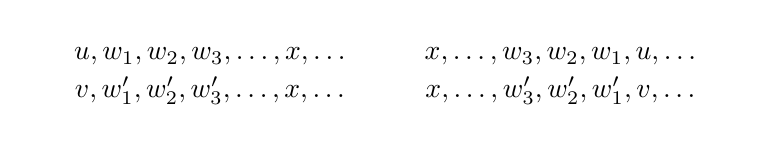
\begin{tikzpicture}
    \matrix(dict)[matrix of nodes,%below=of game,
        nodes={align=center,text width=12em,text height=0.5em},
        %row 3/.style={nodes={text height =1em}},
        %column 1/.style={nodes={text width=10cm,align=right}}
    ]{
        $u, w_1, w_2, w_3, \dots, {x}, \dots$ & $x, \dots, w_3, w_2, w_1, u, \dots$ \\
       $v, w^\prime_1, w^\prime_2, w^\prime_3, \dots,{x}, \dots$  & $x, \dots, w^\prime_3, w^\prime_2, w^\prime_1, v, \dots$ \\
       %(a): walk starting from u and v & (b) reversed walks starting from x \\
       %(a) & (b) \\
    };
\end{tikzpicture}
\end{filecontents*}
\begin{figure}[t]
\centering
\label{fig:graph1}
\resizebox{!}{!}{\begin{tikzpicture}
    \matrix(dict)[matrix of nodes, %below=of game,
        nodes={align=center,text width=20em,text height=5em},
        %row 3/.style={nodes={text height =1em}},
        %column 1/.style={nodes={text width=10cm,align=right}}
    ]{
        $u, w_1, w_2, w_3, \dots, {x}, \dots$ & $x, \dots, w_3, w_2, w_1, u, \dots$ \\
       $v, w^\prime_1, w^\prime_2, w^\prime_3, \dots,{x}, \dots$  & $x, \dots, w^\prime_3, w^\prime_2, w^\prime_1, v, \dots$ \\
       %(a): walk starting from u and v & (b) reversed walks starting from x \\
       %(a) & (b) \\
    };
\end{tikzpicture}
}
\caption{The left are two walks starting from $u$ and $v$ respectively, first meeting at $x$; the right are reversed walks starting from $x$, passing $u$ and $v$ respectively.}\label{fig:one}
\end{figure}

We first give the definition of \emph{reversed walk} as the reversed vertex sequence of the random walk defined in Section \rom{3}.
It is easy to see that there is a one-to-one correspondence between the original random walk and its reverse walk.
Recall in the random walk model interpretation of SimRank, random walks are generated by following the in-edges of the $G$.
 Accordingly, a reverse walk can be generated in the similar way  by following the out-edges.
As a result, the transition probability  in a reversed walk should  be rewritten as:
\begin{equation}
Pr(X_i=v|X_{i-1}=v_{i-1}) = \left\{
        \begin{array}{ll}
	\frac{1}{|I(v_{i})|}, & \quad (v_{i-1}, v_i) \in E; \\
	0,  &\quad otherwise.
        \end{array}
    \right.
	\label{eq:eight}
\end{equation}

From Eq. (\ref{eq:seven}) we see  that the probability of a random walk and its reversed walk are exactly the same.
Given the definition of reverse walk, we  have the following observation:
\begin{observation}
Suppose two random walks starting from $u$ and $v$ respectively, say $W_u$ and $W_v$, met at vertex $x$ after following in-edges for $l$ steps. 
Then if we start from $x$ and follow the out-edges in the graph to generate the set of all possible reversed walks of length $l$, reversed walks of $W_u$ and $W_v$ must be in it.
\end{observation}
For example, in Fig. \ref{fig:one} the left two walks are $W_u$ and $W_v$, and the right are the corresponding two reversed walks starting from $x$, passing $u$ and $v$ respectively. 
Observation 1 says that if the left two walks do exist in the graph topology, then their reversed walks on the right always exist.

Motivated by this, and because of the one-to-one correspondence between reversed walk and random walk, SimRank can be computed based on reversed walks. 
The benefit here is that although the time costs of generating random walks and reversed walks are almost equal, 
the number of vertices starting from which we need to generate reversed walks could be reduced greatly
based on the following observation:

\begin{observation}
Let $W_u=uw_1w_2\dots w_l$ be a  master walk.
Then slave walks with length $l$ could only meet with $W_u$ at one of $\{w_1, w_2, \dots, w_l\}$.
In other words, If we denote by $Nei$ the set of vertices reachable from $u$ in $k$ steps by following in-edges, it suffices to generate reversed walks starting from vertices in $Nei$ rather than $V$ to compute $s(u,*)$.
\end{observation}

The  correctness of this observation is evident. 
Based on the two observations, it is easy to see that now the total  number of reversed walks needed  is $O(|Nei|d^k)$ rather than $O(nd^k)$. 
In fact, $|Nei|$ is roughly $O(d^k)$, which is much smaller than $n$ and is independent of the scale of the underneath graph.
This guarantees efficiency when handling huge web graphs. 

So now we give our new algorithm flow. 
We first generate master walks of length up to $k$ and update the reachable vertex set $Nei$ along the way.
These master walks are carefully recorded and will be shared  by other vertices  in the matching process later.
Then for each vertex in $Nei$, we take it as starting point and generate all slave reversed walks. 
Note that master walks are generated by following in-edges of the graph, while slave walks move along out-edges.
In the following subsections, we discuss for each master walk, how we can find all its matching slave walks and finally compute $s(u, *)$ based on their meeting probabilities.

\subsection {More Compact Representation of Walks}
\iffalse
Because all reversed walks existing in the topology of the input graph are generated no matter whether they finally contribute to the final similarities or not, the amount of walks is huge.
To be more precise Specifically, if the cardinality of neighborhood of query vertex $u$ is $C$, then a total of $Cd^k$ walks will be generated. 
Thus,  to efficiently compute SimRank, we need to consider the following factors: 1)compact representation of walks, which will save memory; and 2)fast search of matching pairs, which is closely related to the overall performance. 
\fi
Although the number of reversed walks needed has been reduced, it still grows exponentially with the average in-degree $d$.
Storing so many reversed walks is costly.
Besides, there also exist redundancies as  lots of walks share common subsequences.
For instance, any prefix or suffix of the vertex sequence of a walk could also form another walk.
%For example, in the Path-Tree used in \cite{li2010fast} as shown in Fig. \ref{fig:two}(b), same vertex in the input graph could appear multiple times in different branches and at different levels. 

Our method  addresses this problem and do as follows. 
For an arbitrary vertex $v$ in the graph, we do not  store  reversed walks  in any specially designed data structure at all. 
Instead, starting from $v$ we let a surfer walk  $k$ steps by following the out-edges of the graph and collect a portion of the input graph --- a {\em neighborhood} of $v$ denoted by $N_{G}(v, k)$.
Formally, $N_{G}(v, k)$ is an induced subgraph formed by all the vertices that are up to $k$ steps away from $v$. 
For example, Fig. \ref{fig:two}(a) shows a neighborhood of vertex $v$. 
Its corresponding Path-Tree representation is shown in Fig. \ref{fig:two}(b). 
The vertex in gray is the  query vertex  $u$. 
Note that $N_{G}(v, k)$ is itself a compressed representation of all the reversed walks, and its graph structure is much more compact than the Path-Tree structure.

We pay special attention to low space complexity because in distributed environments, the process of generating (reversed) walks will inevitably incur network communication overhead since a single computing node has no random access to  the whole graph.
 But in most cases,  data communication via network is one of the leading factors that degrade performance of distributed applications.
 In the next subsection, we will show that although the information of  all walks is hidden in a compact neighborhood, we can still  achieve fast matching of walks.
 
\begin{filecontents*}{temp2.tikz}
		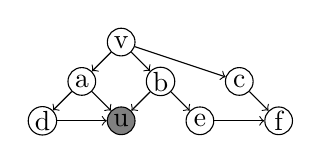
\begin{tikzpicture}[baseline=0pt]
			\begin{scope}[every node/.style={circle,draw,inner sep=0.5pt,minimum size=10pt}, treenode/.style = {circle,draw,inner sep=0.5pt,minimum size=10pt,fill=gray}]
			    \node (d) at (0,0) {d};
			    \node [treenode] (u) at (1,0) {u};
			    \node (e) at (2, 0) {e};
			    \node (f) at (3,0) {f};
			     \node (a) at (0.5, 0.5) {a};
			    \node (b) at (1.5, 0.5) {b};
			    \node (c) at (2.5, 0.5) {c};
			    \node (v) at (1, 1) {v};
			\end{scope}
			\begin{scope}[
			             every node/.style={fill=black,circle},
			              every edge/.style={draw=black}]
			    \path [->] (v) edge  (a);
			    \path [->] (v) edge  (b);
			    \path [->] (v) edge  (c);
			    \path [->] (a) edge  (d);
			    \path [->] (a) edge  (u);
			    \path [->] (b) edge  (e);
			    \path [->] (b) edge  (u);
			    \path [->] (c) edge  (f);
			    \path [->] (d) edge  (u);
			    \path [->] (e) edge  (f);
			\end{scope}
		\end{tikzpicture}
\end{filecontents*}
\begin{filecontents*}{temp3.tikz}
		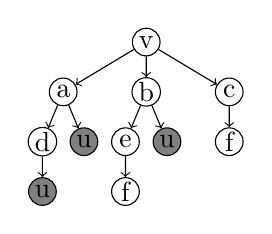
\begin{tikzpicture}[baseline=0pt,->,
		level/.style={sibling distance = 3em/#1,level distance = 1.8em}, 
		interestnode/.style = {circle,draw,fill=gray,inner sep=0.5pt,minimum size=10pt},
		treenode/.style = {circle,draw,inner sep=0.5pt,minimum size=10pt}] 
		\node [treenode] {v}
		    child{ node [treenode] {a} 
		             child{ node [treenode] {d} 
									child{ node [interestnode] {u}}			
		            }
		            child{ node [interestnode] {u}}                    
		    }
		    child{ node [treenode] {b}
		            child{ node [treenode] {e} 
									child{ node [treenode] {f}}			
		            }
		            child{ node [interestnode] {u}}
		    }
		    child{ node [treenode] {c}
		    	  child{ node [treenode] {f} 
		     }
			  }
		; 
		\end{tikzpicture}
\end{filecontents*}

\begin{figure}[t]
    \centering
    \begin{subfigure}[b]{0.48\linewidth}        %% or \columnwidth
        \centering
        \label{fig:two:one}
	\resizebox{!}{!}{  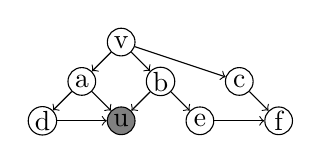
\begin{tikzpicture}[baseline=0pt]
   \begin{scope}[every node/.style={circle,draw,inner sep=0.5pt,minimum size=10pt}, treenode/.style = {circle,draw,inner sep=0.5pt,minimum size=10pt,fill=gray}]
       \node (d) at (0,0) {d};
       \node [treenode] (u) at (1,0) {u};
       \node (e) at (2, 0) {e};
       \node (f) at (3,0) {f};
        \node (a) at (0.5, 0.5) {a};
       \node (b) at (1.5, 0.5) {b};
       \node (c) at (2.5, 0.5) {c};
       \node (v) at (1, 1) {v};
   \end{scope}
   \begin{scope}[
                every node/.style={fill=black,circle},
                 every edge/.style={draw=black}]
       \path [->] (v) edge  (a);
       \path [->] (v) edge  (b);
       \path [->] (v) edge  (c);
       \path [->] (a) edge  (d);
       \path [->] (a) edge  (u);
       \path [->] (b) edge  (e);
       \path [->] (b) edge  (u);
       \path [->] (c) edge  (f);
       \path [->] (d) edge  (u);
       \path [->] (e) edge  (f);
   \end{scope}
  \end{tikzpicture}
}
	\caption{$N_G(v, 4)$.}
	\label{fig:figure2:figure1} \end{subfigure}
    \begin{subfigure}[b]{0.48\linewidth}        %% or \columnwidth
     \centering
	\resizebox{!}{!}{  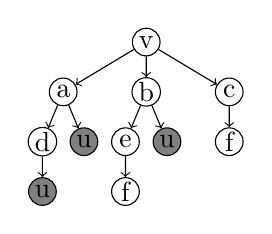
\begin{tikzpicture}[baseline=0pt,->,
  level/.style={sibling distance = 3em/#1,level distance = 1.8em},
  interestnode/.style = {circle,draw,fill=gray,inner sep=0.5pt,minimum size=10pt},
  treenode/.style = {circle,draw,inner sep=0.5pt,minimum size=10pt}]
  \node [treenode] {v}
      child{ node [treenode] {a}
               child{ node [treenode] {d}
         child{ node [interestnode] {u}}
              }
              child{ node [interestnode] {u}}
      }
      child{ node [treenode] {b}
              child{ node [treenode] {e}
         child{ node [treenode] {f}}
              }
              child{ node [interestnode] {u}}
      }
      child{ node [treenode] {c}
         child{ node [treenode] {f}
       }
     }
  ;
  \end{tikzpicture}
}
	\caption{Path-tree of $N_G(v, 4)$.}
	\label{fig:figure2:figure2}
    \end{subfigure}
    \caption{(a) A neighborhood of $v $.  (b) The corresponding Path-Tree representation of the neighborhood.}
    \label{fig:two}
\end{figure}

\subsection {Faster Matching Process}
After each vertex in $Nei$ collects all reversed walks starting from itself, we need to match them with the master walks to compute the final SimRank score.
Assume that all master walks can be accessed by all vertices.
Note that each vertex is responsible for the reversed walk collections of his own, so the whole computation can be  distributed across the cluster easily.
To ease presentation, we take vertex $v$ as an example.
In the matching process, only the reversed walks that share the first common vertex $v$, and differ in all remaining vertex sequences with the master walk are of our interest.
%Any other pairs not satisfying this property would not contribute to computation of SimRank.
For example,  in Fig. \ref{fig:two}(b) paths $vau$ and $vbe$ are  a pair of meeting walks which contributes to $s(u, e)$. 
Meeting walks of $vau$ also include  $vbu$ and $vcf$.
But $vad$ and $vau$ are not meeting pair because they first meet at vertex $a$ rather than $v$ (actually,  in a distributed environment their contribution will be recognized by $a$ somewhere else).
These observations immediately tell us that,  if the query vertex $u$ resides at some level of the Path-Tree of the neighborhood, then all other vertices $w$ at that level satisfying $LCA(u, w)=v$ will contribute to $s(u,w)$ by  $c^{l}Pr(W_u)Pr(W_w)$, where $LCA$ means the Lowest Common Ancestor,  $W_u$ and $W_v$ are the reversed walks corresponding  to the root-to-node path formed by $w$ and $v$ in the tree.
%For example, In  Fig. \ref{fig:two}(b), $v, a, u$  resides in the leftmost subtree of root $v$. 
%Any path of the same length in that subtree will not interest us, because they meet with $v,a,u$ at vertex $a$ instead of $v$ for the first time.
%On the other hand, any other reversed walks($v,b,e$; $v,b,u$; $v,c,f$) in other subtrees will contribute to our final SimRank computation.

%To find the matching reversed walks of a master walk of length $l$, 
We search for all  meeting pairs by  Depth First Searching (DFS) the neighborhood starting from $v$. 
During DFS,  the probability  of the root-to-node path so far is maintained. 
When the recursion depth approaches $l$, the length of the matched master walk,  DFS procedure stops and  the probability of the corresponding reversed walk is recorded in a global hash map.
When we go on to match reversed walks of length $l+1$,  we no longer need to start DFS from $v$ anymore. 
Because probabilities of  reversed walks shorter than $l+1$ could have been recorded before.
For example, in  Fig. \ref{fig:two}(b) the only matching walks of $vadu$  is $vbef$. 
To get its probability, we only need to choose the third vertex $e$ as the staring point of DFS, because the probability of $vbe$ has been recorded when searching for the meeting walks of  $vau$. 

It is not hard to see that our way of matching is a Dynamic Programming approach. 
We use memorization to avoid recomputing overlapping subproblems.
The details are shown in Algorithm \ref{alg:two}.
Procedure LevelMatch shows how a vertex $v$ computes meeting probabilities for master walks of length $l$.
Among the  parameters,
 $W_l$  is a collection of master walks of length $l$.
  $N$ is the neighborhood of $v$.
 %$M_l$ the previous memorized $M_{l^\prime}$ 
 $M_{l^\prime}$ is the previous memorized meeting probabilities for master walks of length $l^\prime$.
 In detail, $M_{l^\prime}$ is a hash map composed of $(key, value)$ pairs, where $key$ could be one of  the neighbors of $v$ in $N$,  and $value$ is a list of pairs each representing the ending vertex and probability of a matching reversed walk  belonging to the subtree with root $key$.
 Similarly $M_l$ is an empty hash map to be filled for $W_l$.
 The last parameter $\delta$ is the probability threshold we will describe in the following subsections.
We first loop the master walk $p$ in $W_l$, and get to know  in which subtree $p$ resides (line 2-3).
Then we start to DFS all other different subtrees if $M_l$ contains no information about that subtree (line 4).
If $M_{l^\prime}$ does not contain information of that subtree, we start DFS right from its root (line 5-6).
Otherwise, we choose to start DFS from those vertices recorded in $M_{l^\prime}$ (line 8-10).
Procedure DFS show the detailed search process. 
We first check if we can terminate the search process early, which will be discussed in detail in next subsection (line 13-15).
Then we check if the depth limit of DFS is reached. If so we stop there and record the probability (line 16-17).
Otherwise, we go on to DFS the next level (line 19-20).
By invoking LevelMatch for all $W_l$ ($l \leq k$), we can compute meeting probabilities  efficiently.

\begin{figure}
\begin{algorithm}[H]
\captionof{algorithm}{Dynamic Programming Path Matching}
\label{alg:two}
\begin{algorithmic}[1]
\Procedure{LevelMatch}{$W_l, N, v, M_{l^\prime}, M_l, \delta$}
	\For {$p \in W_l$}
		\State {$br \gets$ second last vertex of $p$};
			\For {$t \in (v_N.neighbors - br)$ \& $t \notin M_l$}
				
					\If {$!M_{l^\prime}$.contains$(t)$}
						\State \parbox[t]{\dimexpr\linewidth-\algorithmicindent} {\Call{DFS}{$N, t, l, M_l,\delta, t, 1, 1$};}	
					\Else 
						\For {$w \in M_{l^\prime}$}
							\For {$nei \in w_N.neighbors$}
								\State \parbox[t]{\dimexpr\linewidth-\algorithmicindent}{\Call{DFS}{$N, nei, l,M_l,\delta,br,w.mul, l^\prime$};}
							\EndFor
						\EndFor
					\EndIf			
				
			\EndFor
	\EndFor
	\State \textbf{return} $M_l$.
	%\State \textbf{return} $results$.
\EndProcedure
\Procedure{DFS}{$N, v, l, M,\delta ,br ,mul,depth$}
	\State {$mul \gets mul * v_N.indegree$};
	\If {$mul > \delta$}
		\State \textbf{return;} \Comment{Early termination.}
	\EndIf
	\If {$depth = l$}
		\State {add $(v, mul)$ to $M(br)$};  \Comment{Record  probability.} %to the branch it resides in.}
	\Else
		\For {$nei \in v_N.neighbors$}
			\State \parbox[t]{\dimexpr\linewidth-\algorithmicindent} {\Call{DFS}{$N, nei, l, M,\delta, br,mul$, $ depth+1$};}
		\EndFor
	\EndIf
	\State \textbf{return} $M$.
\EndProcedure
\end{algorithmic}
\end{algorithm}
\end{figure}
\subsection{Early Termination of Walks}
Many real-world graphs are scale-free \cite{li2005towards}, which means that a small portion of the vertices in the graph have very large degrees. 
Our algorithm could suffer a lot from the presence of these high degree vertices, since higher degree means more splits of walks.
%If the probability of a walk containing many high degree vertices is already small enough,  further advance of the walk will cost a lot of computation but contribute little practical information for the result similarity. 
Thus, we adopt probability sieve \cite{lizorkin2008accuracy} to filter out the walks  whose probability is already small enough caused by containing many high degree vertices.
The filtered walks will no longer advance any further because the contribution of subsequent walks are  insignificant. 
%Once a walk reaches a new vertex, its probability will be multiplied by the reciprocal of the in-degree of the landing vertex. 
%If the new probability is below a small threshold $\delta$, the walk will terminate at that vertex.
%Any further walk that contains this path as prefix will be ignored, because their 
The value of the probability threshold $\delta$ can be set manually to achieve a balance between tolerance of accuracy loss and improvement of computing efficiency.
Note that this optimization generally can be applied to every walk generation process, e.g.,  in line (13-15) of the DFS procedure of Algorithm \ref{alg:two}.

\subsection{sssSimRank: Putting it All Together}
Given  all the techniques that we described in the previous subsections, we now list the framework of our sssSimRank algorithm as the following phases:
\begin{enumerate}
\item Find the set of vertices $Nei$ that are reachable from  $u$ by following in-edges, and at the same time maintain corresponding master walks. All master walks are then broadcast to all machines in the cluster;
\item Each vertex in $Nei$ collects its neighborhood by following out-edges;
\item Each above vertex then computes meeting probabilities based on its own copy of master walks and  the reversed walks extracted from its own neighborhood; 
\item All meeting probabilities scores are aggregated to get the final $s(u, *)$.
\end{enumerate}

In a typical distributed environment, most of the network communication happens in phase 1 and especially phase 2, as neighbor information needs to be exchanged between all machines.
Phase 4 will also incur some communication cost.
Most of the computations, including searching for  meeting walks and calculating their  probabilities, are 
conducted locally by each machine in the cluster.

We analyze the complexity  of our algorithm in all respects. 
The total amount of vertices reachable from $u$ is $O(d^{k})$.
For each of the reachable vertices, it has a neighborhood of size $O(d^{k})$ containing structure information of all  $O(d^k)$ reversed walks.
So the total space complexity is  $O(d^{2k})$.
The communication cost involved in Phase 1 and Phase 2 is also $O(d^{2k})$ because at most all walks are transferred.
Phase 3 uses memorization technique to compute meeting probabilities, thus for a single neighborhood at most all $O(d^k)$ reversed walks are matched. 
This leads to a total computation cost of $O(d^{2k})$.
A tight bound of communication cost of phase 4 is hard to give, but we can assert that it only depends on the topology rather than the scale of the graph. In summary, our approach of  computing single-source SimRank is highly efficient and  allows for high parallelism.
 
\section{Implementation on Spark}
In this section, we describe the implementation of sssSimRank  on Spark. 
Note that  phase 1 and phase 2  of our algorithm are quite similar.
In both cases we start from some vertices and find their reachable neighbors.  
The only differences lie  in the number of starting vertices (1 vs. $|Nei|$) and the direction of movement (following in-edge vs. out-edges). 
So we omit phase 1 and explain the other three in detail.


\subsection{Collect Neighborhood}
The process of collecting neighborhood for each vertex $v\in Nei$ is shown in Algorithm \ref{alg:three}.
The algorithm takes 3 input parameter.
 $edgeRDD$ is the RDD of the graph, $u$ is the query vertex, and $k$ is the maximum walk length.
First we convert the graph from plain edge format to adjacent list format (line 2-3).
We then initialize $nbrhdRDD$ from $graphRDD$  by filtering out the vertices not in $Nei$, which contains the one-step neighborhood of each vertex.
 And {\asciifamily cache} is called to persist $nbrhdRDD$ into memory for later iterations (line 4).
At the very beginning, the neighborhood only covers the out-neighbors of the vertex.
In the following iterations, the neighborhood will expand larger by advancing a step further from the out-most vertices. 
$nbrRDD$ is the RDD that contains the out-most vertices of neighborhood of each vertex. 
It is initialized as out-neighbors of $u$ from $graphRDD$ (line 5).
We now begin to expand all the neighborhoods iteratively.
In each iteration, first the out-most neighbors are updated by joining the underneath graph (line 7-8).
Then the new out-most neighbors are transferred to neighborhoods who can reach them (line 9-10).
Finally, we get the neighborhood for each starting vertex after $k$ iterations.

\begin{figure}
\begin{algorithm}[H]
\captionof{algorithm}{Collect Neighborhood}
\label{alg:three}
\begin{algorithmic}[1]
	\Procedure{Collect}{$edgeRDD, u, k$}
		\State {$graphRDD \gets edgeRDD$}
		\State {\qquad .{\asciifamily reduceByKey}$()$.{\asciifamily cache}$()$};
		\State {$nbrhdRDD \gets graphRDD$.{\asciifamily map}$()$.{\asciifamily cache}$()$};
		\State {$nbrRDD \gets graphRDD$.{\asciifamily filter}$()$.{\asciifamily cache}$()$};
		\For{$ l =2$ to $k$}
			\State {$nbrRDD \gets  nbrDD$}
			\State {\qquad.{\asciifamily join}$(graphRDD)$.{\asciifamily map}$()$};
			\State {$nbrhdRDD \gets nbrhdRDD$}
			\State {\qquad .{\asciifamily leftOuterJoin}$(nbrRDD)$.{\asciifamily map}$()$};
		\EndFor
	\State \textbf{return} $nbrhdRDD$.
	\EndProcedure
\end{algorithmic}
\end{algorithm}
\end{figure}

\subsection{Compute and Aggregate Meeting Probabilities}
After all neighborhoods of each starting vertex have been collected, we begin to match all master walks and slave walks. 
The details are listed in Algorithm \ref{alg:four}.
The algorithm takes 4 parameters.
The first parameter $nbrhdRDD$ is the output of Algorithm \ref{alg:three}, the RDD containing pairs of vertex and its neighborhood.
The second parameter $MW$ is the output of phase 1, i.e., all the master walks starting from $u$.
$MW$ is represented as a  hash map of $(key, value)$ pairs, where $key$ is the ending vertex of each master walk (note that $key \in Nei$), and $value$ is a list of the random walks ending with $key$.
The remaining two parameters are the given query vertex and maximum walk length, respectively.
For each record $(v, nbrhd)$ in $hbrhdRDD$, we invoke LevelMatch in Algorithm \ref{alg:two} to compute meeting probabilities of all meeting walks in  $nbrhd$ for $v$. 
The results are appended into the list $MP$ (line 5-7).
Then all meeting probabilities are emitted by {\asciifamily flatMap} (line 8-9).
%in which each element is a pair, containing the ending vertex of a walk and its corresponding meeting probability (line 7).
%The resulting matched reversed walks $MRW$ is then emitted by {\asciifamily flatMap} (line 7-8). 
In the end,  {\asciifamily reduceByKey} aggregates all the probabilities to form the final SimRank score, which are subsequently collected to the driver program (line 11-12).

\begin{figure}[!t]
\begin{algorithm}[H]
\captionof{algorithm}{Compute SimRank}
\label{alg:four}
\begin{algorithmic}[1]
\Procedure{Compute}{$nbrhdRDD, MW,  u, k$}
	\State {$simRankRDD \gets hbrhdRDD$}
	\State {\qquad .{\asciifamily flatMap}$((v, nbrhd) \Rightarrow\{$}
	\State {\qquad \qquad create $MP$};
	\State {\qquad \qquad \textbf{for} $W_l$ in $MW$ \textbf{do}}
	\State {\qquad \qquad \qquad $M \gets$ \Call{LevelMatch}{$W_l, \dots $}};
	\State {\qquad \qquad \qquad extend $MP$ with all elemetns in $M$};
	\State {\qquad \qquad \textbf{for} $(v, score(u,v))$ in $MP$ \textbf{do}}
	\State {\qquad \qquad \qquad yield $(v, score(u,v))$};
	\State {\qquad $\})$}
	\State {$s(u,*) \gets simRankRDD$.{\asciifamily reduceByKey}$()$.{\asciifamily collect}$()$};
	\State \textbf{return} $s(u, *)$.
\EndProcedure
\end{algorithmic}
\end{algorithm}
\end{figure}

\begin{table}[h]
\renewcommand{\arraystretch}{1.3}
\caption{Description of Datasets}
\label{tab:one}
\centering
\begin{tabular}{|l|r|r|r|r|}
\hline
\textbf{Dataset} & \textbf{\#Nodes} & \textbf{\#Edges} & \textbf{Avg Deg} & \textbf{Size} \\
\hline
p2p-gnutella08 \footnotemark[1]  & {6,301}         & \num{20777}                   & 3.29                & 215.2KB\\
\hline
wiki-vote \footnotemark[2]    & 7,115 	& \num{103,689}                           &14.57                & 1.1MB  \\
\hline
%wiki-talk            & \num{2394385} & \num{5021410}          &2.10                   & 66.5MB\\
%\hline
eu-2005       \footnotemark[3]     & \num{862664}  & \num{19235140 }          & 22.29             & 256.4MB\\
\hline
ljournal-2008  \footnotemark[4] & \num{5363260} & \num{79023142}         & 14.73            &1.2GB\\
\hline
arabic-2005 \footnotemark[5]   & \num{22744080} & \num{639999458}      & 28.14           & 10.9GB\\
%\hline
%twitter-2010    & \num{41652230 } & \num{1468365182} & 26.1GB\\
\hline
\end{tabular}
\end{table}
\section{Experimental Results}
In this section, we evaluate our implementation of  sssSimRank experimentally.
We first describe our running environments, datasets used, and parameter settings.
Then we analyze our results in terms of effectiveness, efficiency and scalability.%in detail.

\begin{figure*}[t]
\centering
\begin{subfigure}[b]{0.32\textwidth}
	\center
	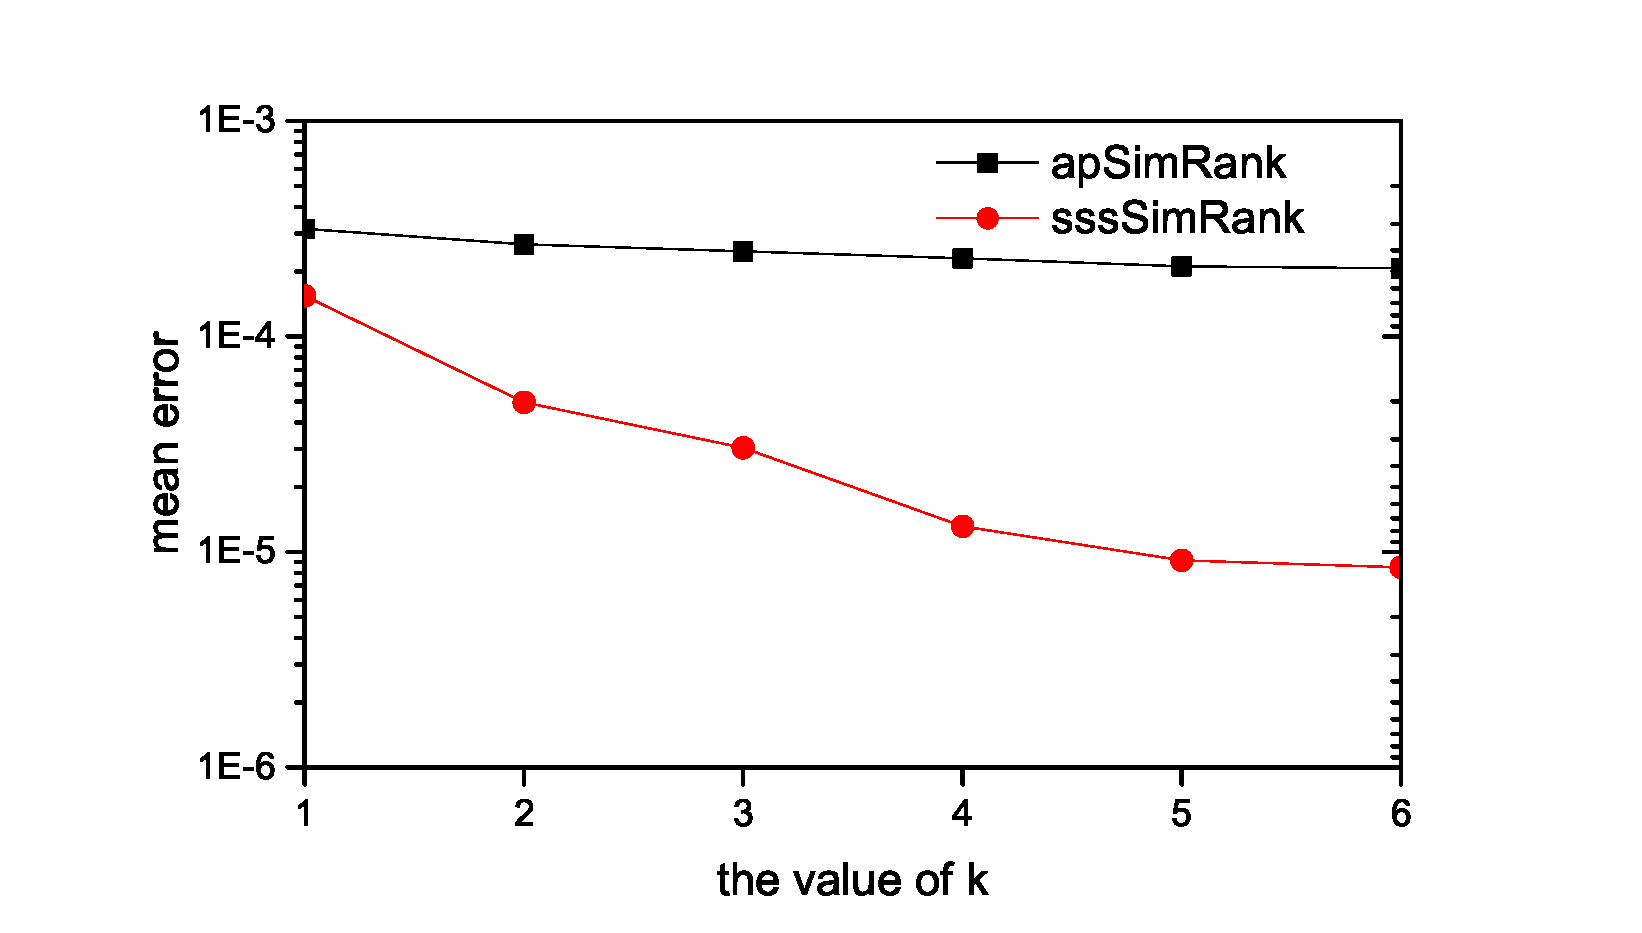
\includegraphics[width=1\textwidth]{resource/graph/accuracy1.eps}
	\caption{Comparison of accuracy   between sssSimRank and apSimRank on p2p-gnutella08.}
	\label{fig:three:a}
\end{subfigure}
%\qquad
\begin{subfigure}[b]{0.32\textwidth}
	\centering
	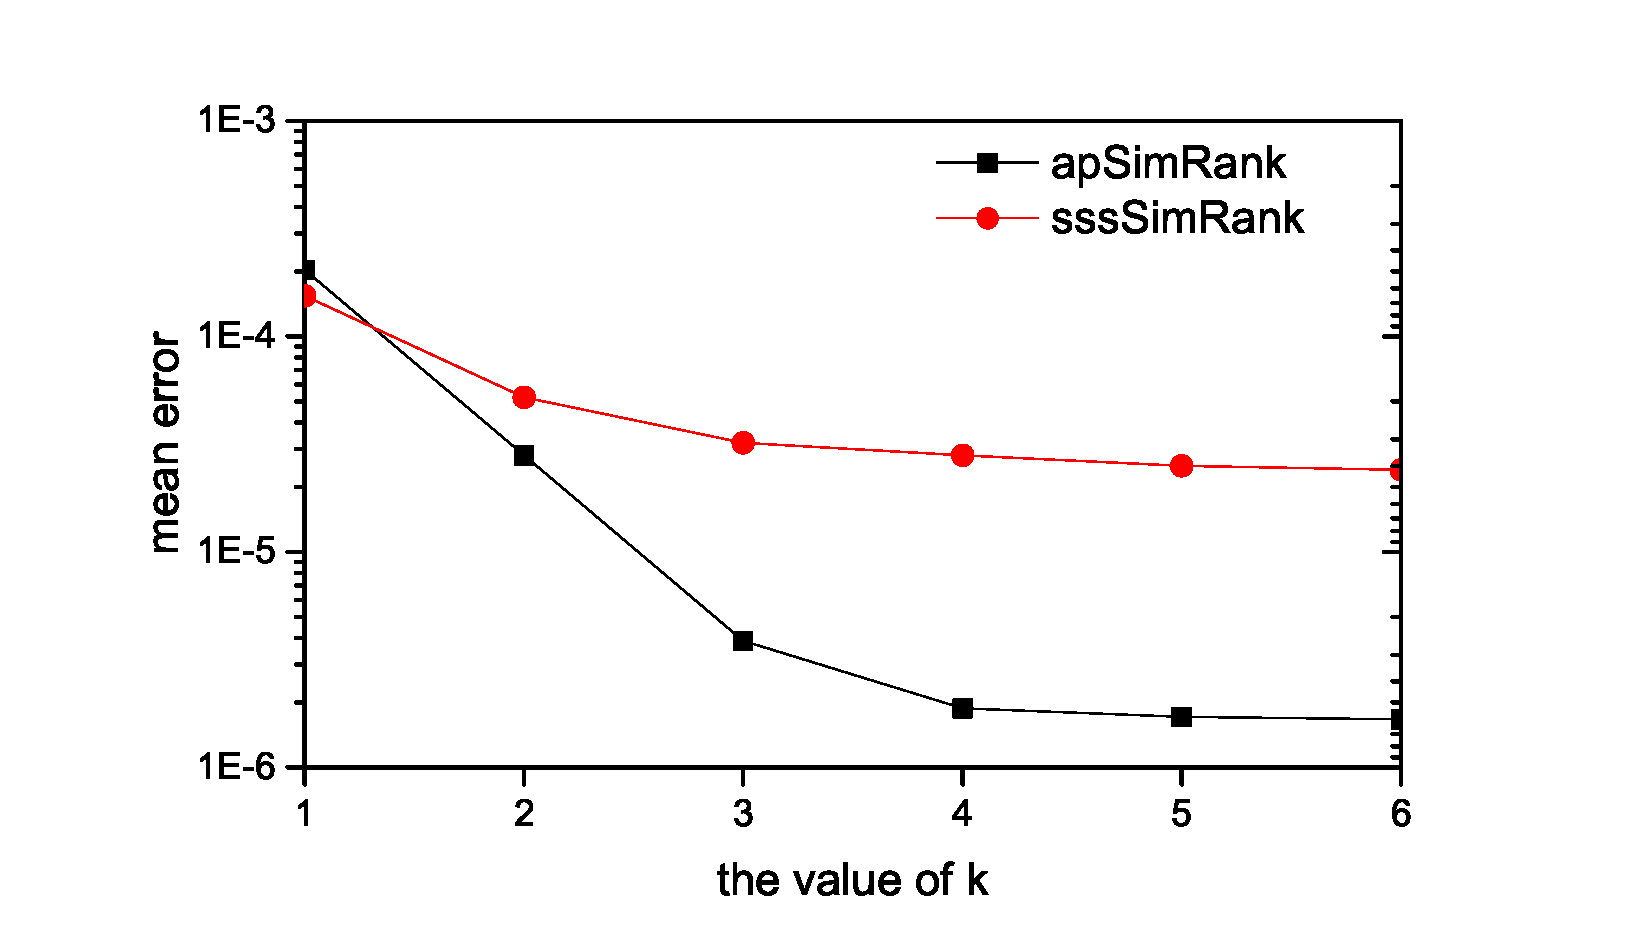
\includegraphics[width=1\textwidth]{resource/graph/accuracy2.eps}
	\caption{Comparison of accuracy   between sssSimRank and apSimRank on wiki-vote.}
	\label{fig:three:b}
\end{subfigure}
%\quad
\begin{subfigure}[b]{0.32\textwidth}
	\centering
	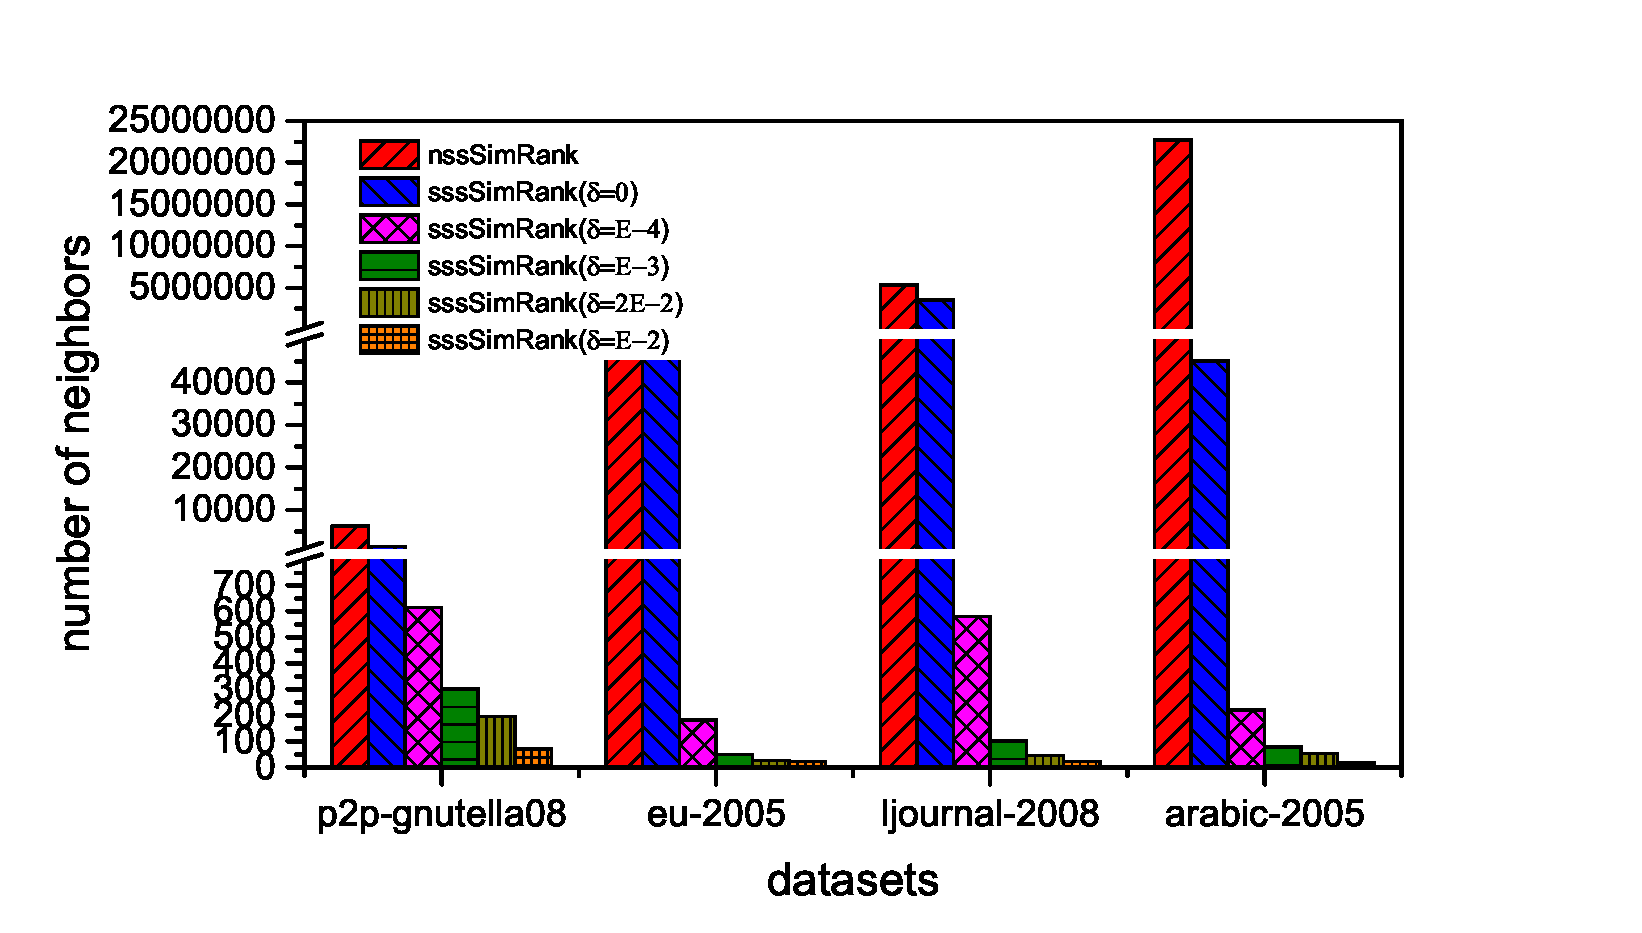
\includegraphics[width=\textwidth]{resource/graph/neighborhoods.eps}
	\caption{Comparison of $|Nei|$ between nssSimRank and sssSimRank with varying probability threshold.}
	\label{fig:three:c}
\end{subfigure}
\medskip
\begin{subfigure}[b]{0.32\textwidth}
	\centering
	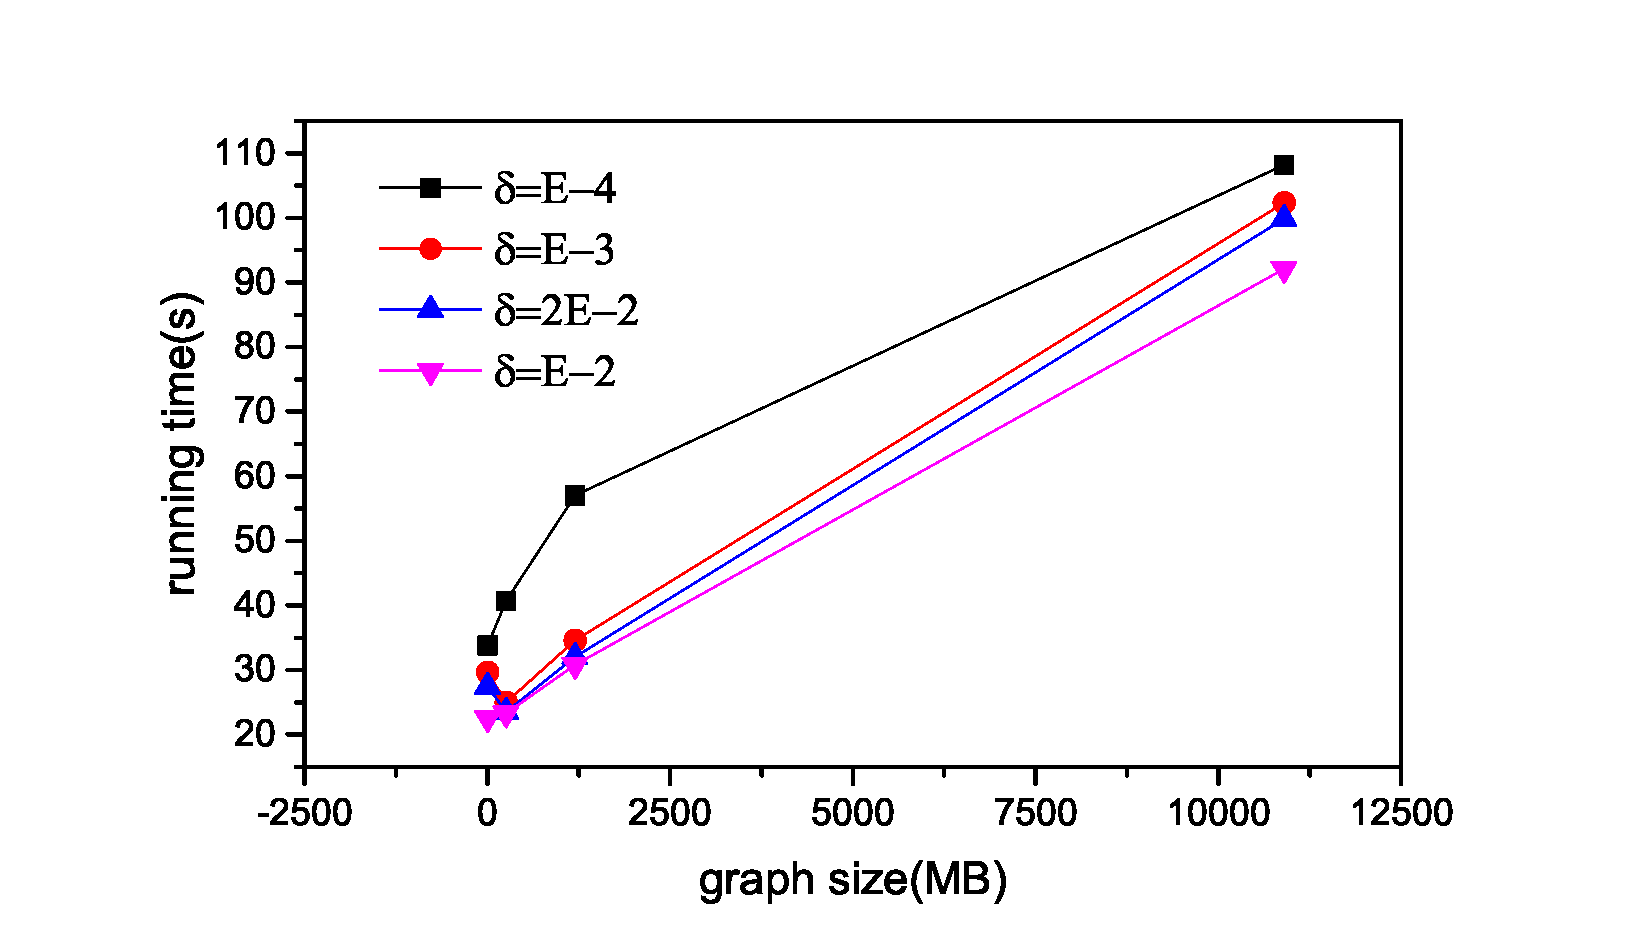
\includegraphics[width=\textwidth]{resource/graph/data_scalability.eps}
	\caption{Running time with varying graph sizes.}
	\label{fig:three:d}
\end{subfigure}
\qquad
\begin{subfigure}[b]{0.32\textwidth}
	\center
	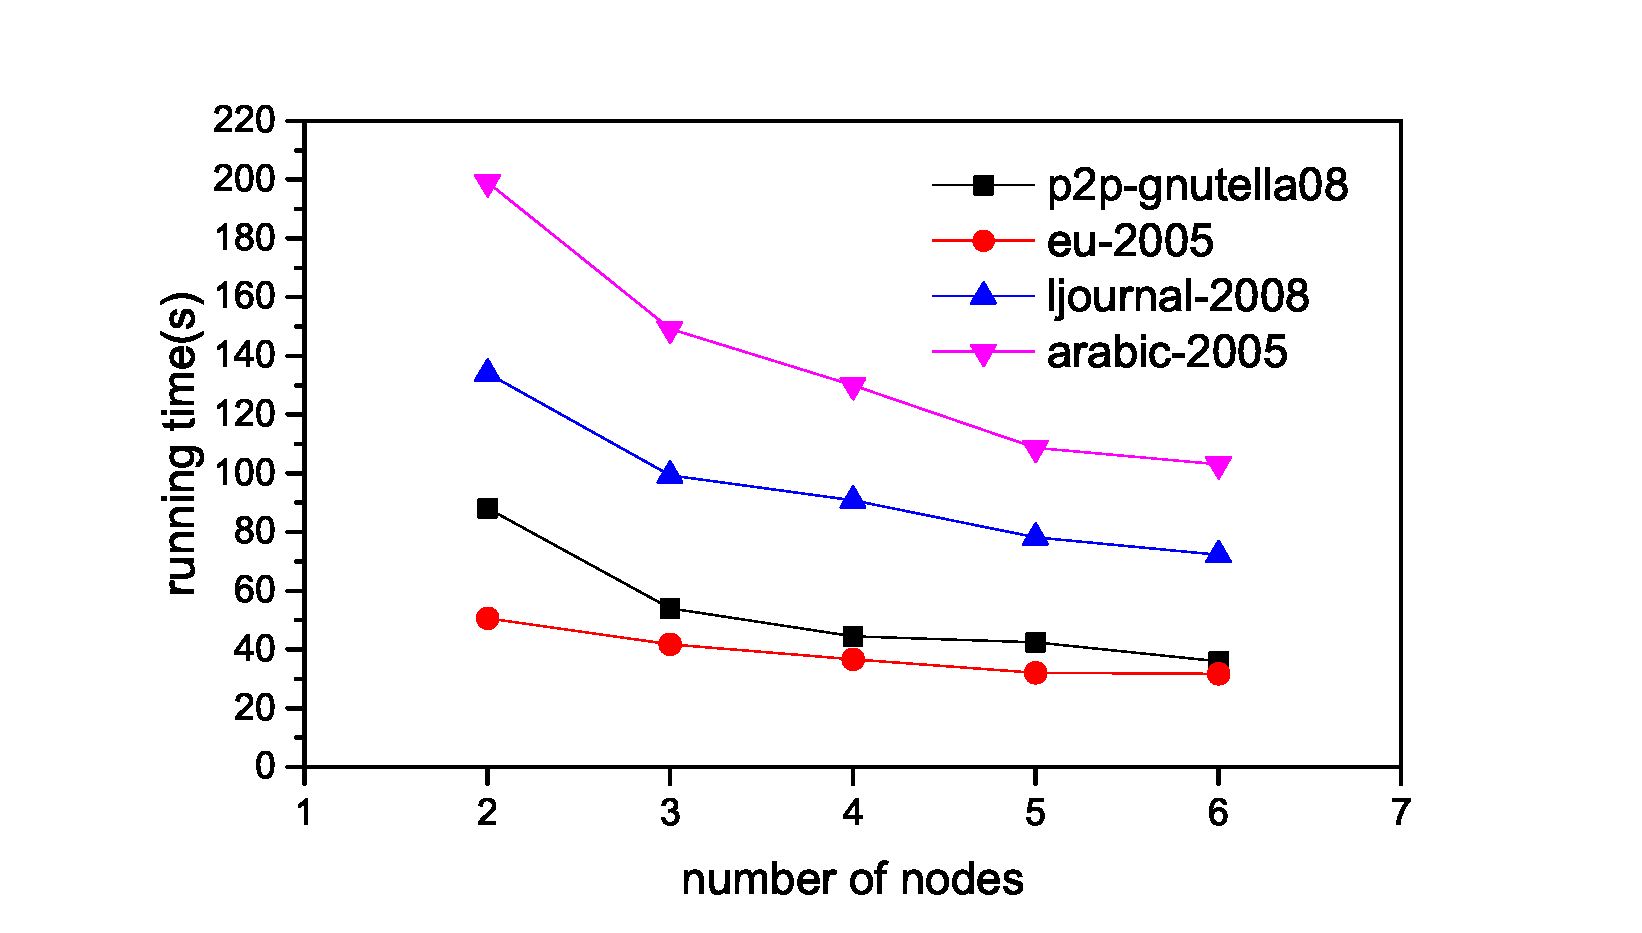
\includegraphics[width=\textwidth]{resource/graph/node_scalability.eps}
	\caption[width=\textwidth]{Running time with varying number of nodes.}
	\label{fig:three:e}
\end{subfigure}
\caption{Results of accuracy loss and convergence rate, efficiency and scalability.}
\label{fig:three}
\end{figure*}
\footnotetext[1]{https://snap.stanford.edu/data/p2p-Gnutella08.html}
\footnotetext[2]{https://snap.stanford.edu/data/wiki-Vote.html}
\footnotetext[3]{http://law.di.unimi.it/webdata/eu-2005/}
\footnotetext[4]{http://law.di.unimi.it/webdata/ljournal-2008/}
\footnotetext[5]{http://law.di.unimi.it/webdata/arabic-2005/}
\subsection {Setup}
\subsubsection{Running Environment}
We do all experiments on a cluster of 6 machines, each has two 12-core Intel Xeon E5-2650 2.10 GHz processors, 64 GB RAM, and 1TB hard disk. 
Each of them are connected via a Gigabit network.
All machines are running Ubuntu 14.04.
The version of Spark and underlying HDFS deployed are 1.6.2 and 2.6.0 respectively.
All machines are configured as slave node, and one of them also plays the role of master node.
Each executor in Spark is allocated with 10GB memory.
\subsubsection{Datasets}
We use 5 real-word datasets of various scales.
The details of each dataset are listed in Table \ref{tab:one}.
Each graph is stored as plain text format,  one edge per line. 
All datasets are uploaded into the HDFS beforehand. 
\subsubsection{Parameters}
As discussed by \cite{lizorkin2008accuracy}, the maximum steps $k$ is determined by $c$ and the accuracy we want.
if we want make the error loss  $s^*(u,v) - s^k(u,v)$ smaller than $\epsilon$, we need to set $k=\lfloor \log_c \epsilon \rfloor$. 
In our experiments, we choose  $\epsilon = 0.01$, which is accurate enough for most real-world applications.
$c$ is set to be 0.5 and as a result,  $k = 6$.

For the optimization technique using threshold to ignore walks with small probabilities, we set $\delta=0.002$.
Notice that here $\delta$ is for a single walk. 
For a pair of meeting walks, the equivalent threshold for the meeting probability would roughly be $\delta^2$ according to Eq. (\ref{eq:five}).
After multiplying a factor of $c^l$,  it will be  extremely small and therefore could be reasonably ignored.

To avoid particularity, all experiments are conducted multiple times with the query vertex chosen randomly from the graph.
If not otherwise specified, for small graphs (< 10MB) we repeat 100 times and present the average results while for large graphs the repetition is 1000.


\subsection{Effectiveness}
We compare the accuracy and convergence rate between all-pair SimRank (apSimRank) and  sssSimRank algorithm.
We  evaluate the effectiveness  by  computing the {\em mean error} $ME = \frac{1}{n}\sum_{v \in V}{|s(u,v) - s^k(u,v)|}$, where $s(u,v)$ is the ground truth given by Eq. (\ref{eq:two}) until convergence, and $s^k(u,v)$ is the output of  algorithms running  $k$ iterations (or within 6 steps). 
The comparison is conducted on two small graphs, p2p-gnutella08 and wiki-vote. 
P2p-gnutella08 is a sparse graph ($d=3.29$) while wiki-vote is much denser ($d=14.57$).
The results are shown in Fig. \ref{fig:three}(a).
We can see that both apSimRank and  sssSimRank converge within 6 iterations.
In Fig. \ref{fig:three}(a), sssSimRank achieves a faster convergence rate, with accuracy loss less than $10^{-4}$ after 3 iterations.   
While in Fig. \ref{fig:three}(b), apSimRank  shows better accuracy.
This is because sssSimRank uses a threshold $\delta$ to filter out walks with very small probabilities, which is particularly effective for scale-free graphs like wiki-vote.
By doing so we  improved efficiency at the cost of  some accuracy.
But such a small accuracy loss ($< 10^{-4}$) is ignorable for most real-world  applications.



\iffalse
\begin{figure}[t]
\centering
  \begin{subfigure}[t]{0.5\textwidth}
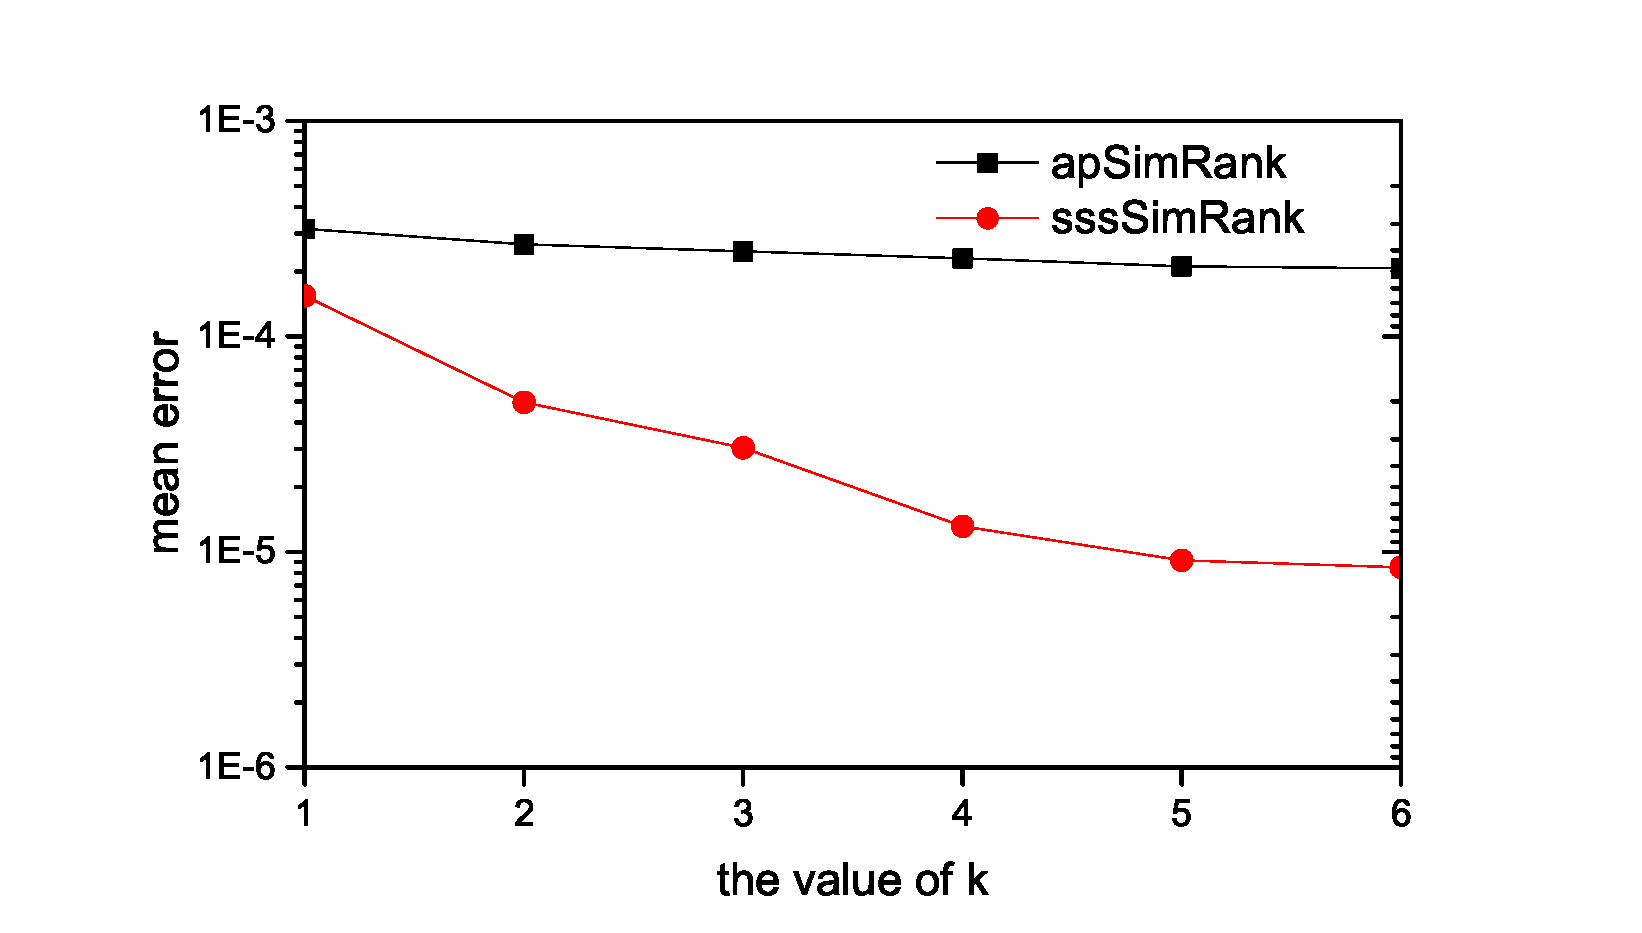
\includegraphics[clip, width=\textwidth]{resource/graph/accuracy1.eps} 
    \caption{Input graph: p2p-gnutella08}
    \label{fig:1}
  \end{subfigure}
  %
  \begin{subfigure}[t]{0.5\textwidth}
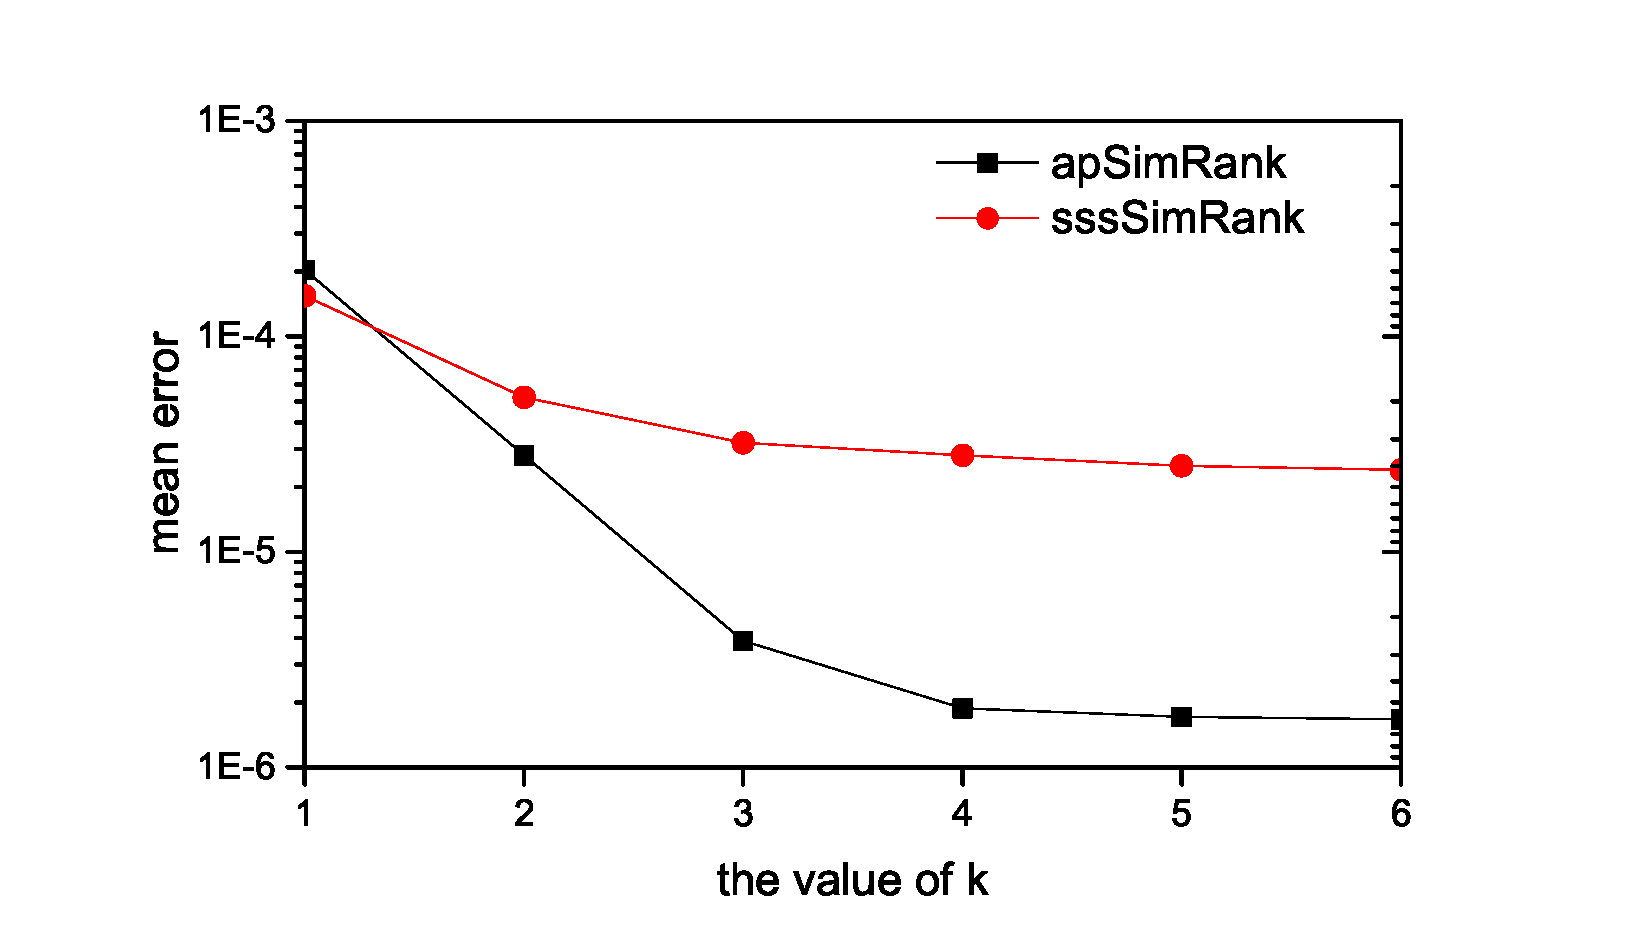
\includegraphics[clip, width=\textwidth ]{resource/graph/accuracy2.eps} 
    \caption{Input graph: wiki-vote}
    \label{fig:2}
  \end{subfigure}
      \caption{Comparison of accuracy loss and convergence rate between sssSimRank and apSimRank.}
    \label{fig:three}
\end{figure}

\begin{figure}[h]
\centering
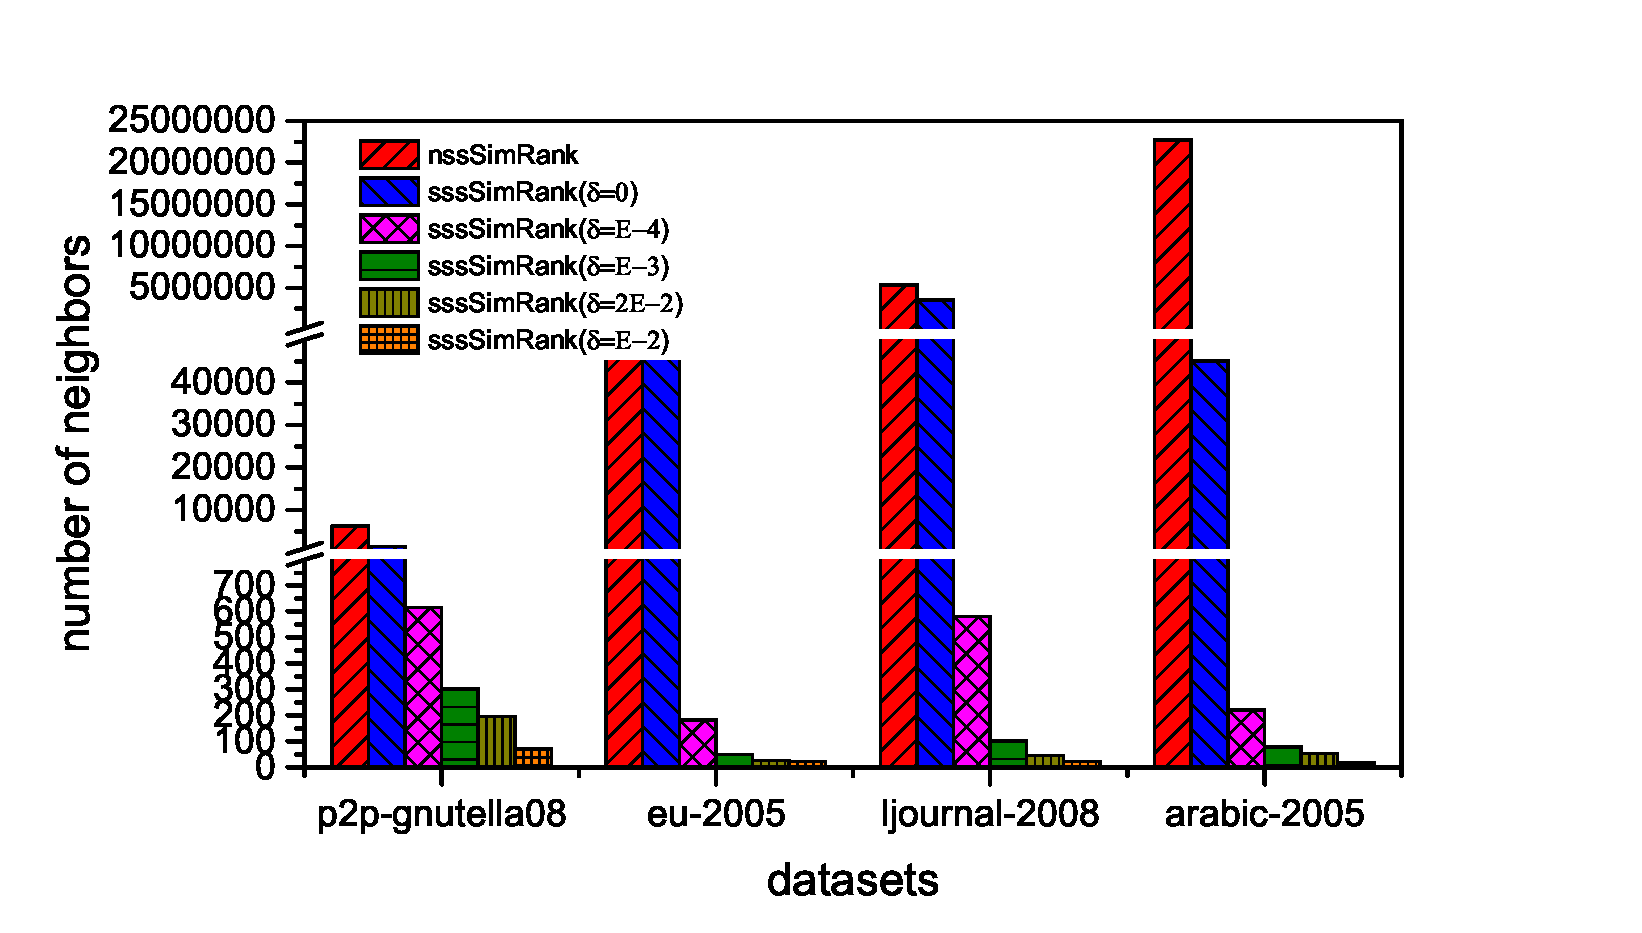
\includegraphics[clip, width=0.5\textwidth ,height=0.2\textheight]{resource/graph/neighborhoods.eps} 
    \caption{Comparison of $|Nei|$ between nssSimRank and sssSimRank with varying probability threshold. }
    \label{fig:four}
\end{figure}
\fi
\subsection{Efficiency}
We implement all-pair SimRank (apSimRank) based on Eq. (\ref{eq:two}), and Naive Single-source SimRank (nssSimRank) based on single-source similarity discussed in \cite{li2010fast}. 
Both of them are implemented as distributed algorithms on Spark. 
We find that a straight comparison between them and our algorithm  on all  graph datasets is impractical  because  computing apSimRank and nssSimRank is extremely time-consuming even for small graphs.
For  apSimRank,  the smallest graph p2p-gnutella08 takes about 2.1 hour to finish.
We think this fact is enough to prove that our algorithm outperforms apSimRank greatly.
For nssSimRank, it takes 1.1 hour. 
Note that the running time of  random-walk-based algorithms mainly depends on the total number of random walks generated, which further depends on the number of neighborhoods. 
Thus, we compare the size of $Nei$ for both nssSimRank and sssSimRank with different $\delta$.
The results are shown in Fig. \ref{fig:three}(c).
In nssSimRank, $|Nei|$ is equal to $n$, because all vertices in the graph need to collect its neighborhood.
In contract, our algorithm reduce $|Nei|$ drastically.
When $\delta$ is 0, which means no probability sieve is used, sssSimRank generates several order of  magnitude (up to 1500x) fewer  neighborhoods.
As $\delta$ becomes larger, which means our probability sieve is more fine-meshed,  number of survivors decreases accordingly. 
Fig. \ref{fig:three}(c)  also indicates that the reduction ratio for eu-2005  and arabic-2005 are higher than that of  p2p-gnutella08  and ljournal-2008.
This shows that probability sieve works better for denser graphs, which is in line with our expectations. 

\subsection{Scalability}
In this section, we investigate the scalability of our proposed algorithm.
The input graphs used are p2p-gnutella08, eu-2005, ljournal-2008 and arabic-2005.
We first evaluate the performance when the data size increases. 
%Maximum random walks length is set as  6.
The running time of sssSimRank with different $\delta$ on the four graphs are shown in Fig. \ref{fig:three}(d).
We can see that our algorithm scales well as the size of  graph increases thousands of times.
Fig. \ref{fig:three}(d) also suggests that for a fixed graph, a larger $\delta$ will bring about larger amount of walks, causing increased running time.

We also evaluate the performance when the number of computing machines increases.
The number of computing nodes increases from 2 to 6.
The configurations for all datasets are the same, with $k=6$ and $\delta=1E$-4.
We adopt a small $\delta$ to increase the overall computing load, because with small workload Spark initialization will dominate the running time.
The results are shown in Fig. \ref{fig:three}(e).
The  nature  of  the  curve  indicates  that,  as  the  number of nodes increases  the running  time decreases as  expected for strong  scalability.
\iffalse
\begin{figure}[t]
\centering
  \begin{subfigure}[t]{\linewidth}
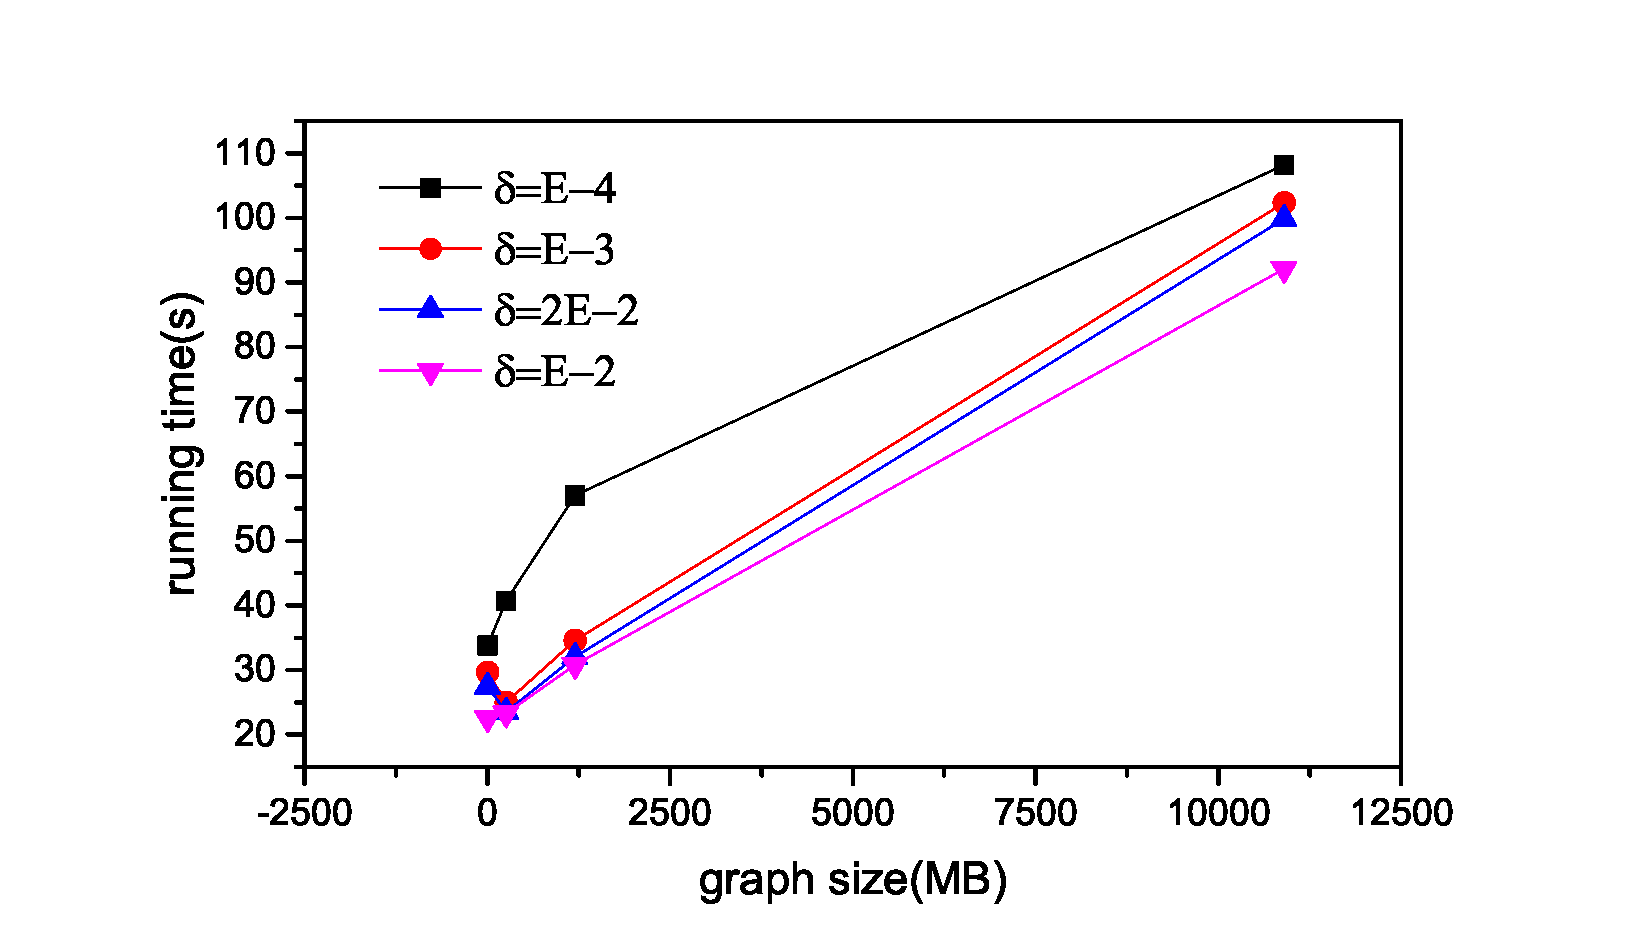
\includegraphics[clip, width=\textwidth]{resource/graph/data_scalability.eps} 
    \caption{Running time with different graph sizes.}
    \label{fig:1}
  \end{subfigure}
  \begin{subfigure}[t]{\linewidth}
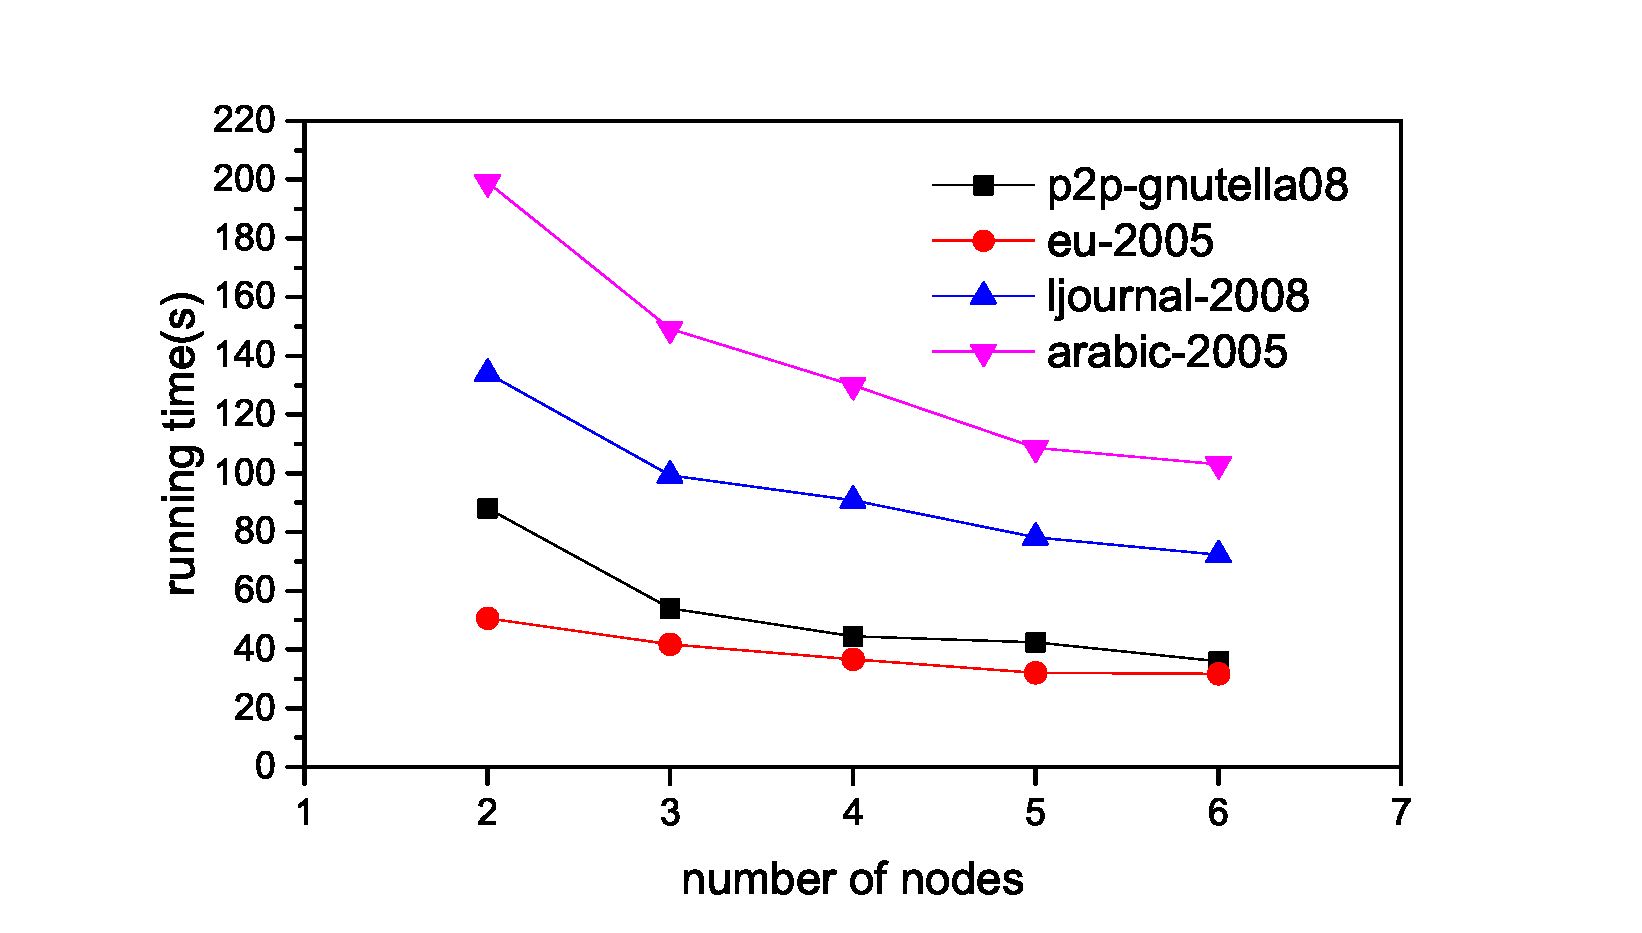
\includegraphics[clip, width=\textwidth ]{resource/graph/node_scalability.eps} 
    \caption{Running time with different number of nodes.}
    \label{fig:2}
  \end{subfigure}
      \caption{Data scalability and node scalability. }
    \label{fig:five}
\end{figure}
\fi

\section{Conclusion}
We have proposed and implemented a highly parallelizable algorithm, sssSimRank, for the computation of single-source SimRank. 
Our algorithm is based on the random walk model. 
It achieves good performance by minimizing the number of walks, compressing representation of intermediate data, and fast matching via dynamic programming.
Experimental results verify the effectiveness, efficiency of our approach. 



% conference papers do not normally have an appendix


% use section* for acknowledgment
\section*{Acknowledgment}
%Their constructive comments and suggestions are very helpful. 
This paper is partly funded by National Science and Technology Major Project of the Ministry of Science and Technology of China under grant 2011ZX05035-004-004HZ.
We  thank the  reviewers for helping us refine this paper. 
% The corresponding author of this paper is Jie Tang.
%We would like to thank the anonymous reviewers for helping us refine this paper. 
%Their constructive comments and suggestions are very helpful. 
%This paper is partly funded by National Science and Technology Major Project of the Ministry of Science and Technology of China under grant 2011ZX05035-004-004HZ. 
%The corresponding author of this paper is Tang Jie.


% trigger a \newpage just before the given reference
% number - used to balance the columns on the last page
% adjust value as needed - may need to be readjusted if
% the document is modified later
%\IEEEtriggeratref{8}
% The "triggered" command can be changed if desired:
%\IEEEtriggercmd{\enlargethispage{-5in}}

% references section

% can use a bibliography generated by BibTeX as a .bbl file
% BibTeX documentation can be easily obtained at:
% http://mirror.ctan.org/biblio/bibtex/contrib/doc/
% The IEEEtran BibTeX style support page is at:
% http://www.michaelshell.org/tex/ieeetran/bibtex/
%\bibliographystyle{IEEEtran}
% argument is your BibTeX string definitions and bibliography database(s)
%\bibliography{IEEEabrv,../bib/paper}
%
% <OR> manually copy in the resultant .bbl file
% set second argument of \begin to the number of references
% (used to reserve space for the reference number labels box)

\bibliographystyle{IEEEtran}
\bibliography{my}

\iffalse

\begin{thebibliography}{1}

\bibitem{fouss2007random}
F.~Fouss, A.~Pirotte, J.-M. Renders, and M.~Saerens, ``Random-walk computation
  of similarities between nodes of a graph with application to collaborative
  recommendation,'' \emph{IEEE Transactions on knowledge and data engineering},
  vol.~19, no.~3, pp. 355--369, 2007.

\bibitem{bhattacharya2006entity}
I.~Bhattacharya and L.~Getoor, ``Entity resolution in graphs,'' \emph{Mining
  graph data}, p. 311, 2006.

\bibitem{dean1999finding}
J.~Dean and M.~R. Henzinger, ``Finding related pages in the world wide web,''
  \emph{Computer networks}, vol.~31, no.~11, pp. 1467--1479, 1999.

\bibitem{jaccard1901etude}
P.~Jaccard, \emph{Etude comparative de la distribution florale dans une portion
  des Alpes et du Jura}.\hskip 1em plus 0.5em minus 0.4em\relax Impr. Corbaz,
  1901.

\bibitem{baeza1999modern}
R.~Baeza-Yates, B.~Ribeiro-Neto \emph{et~al.}, \emph{Modern information
  retrieval}.\hskip 1em plus 0.5em minus 0.4em\relax ACM press New York, 1999,
  vol. 463.

\bibitem{dice1945measures}
L.~R. Dice, ``Measures of the amount of ecologic association between species,''
  \emph{Ecology}, vol.~26, no.~3, pp. 297--302, 1945.

\bibitem{jeh2002simrank}
G.~Jeh and J.~Widom, ``Simrank: a measure of structural-context similarity,''
  in \emph{Proceedings of the eighth ACM SIGKDD international conference on
  Knowledge discovery and data mining}.\hskip 1em plus 0.5em minus 0.4em\relax
  ACM, 2002, pp. 538--543.

\bibitem{page1999pagerank}
L.~Page, S.~Brin, R.~Motwani, and T.~Winograd, ``The pagerank citation ranking:
  bringing order to the web.'' 1999.

\bibitem{lizorkin2010accuracy}
D.~Lizorkin, P.~Velikhov, M.~Grinev, and D.~Turdakov, ``Accuracy estimate and
  optimization techniques for simrank computation,'' \emph{The VLDB
  Journal—The International Journal on Very Large Data Bases}, vol.~19,
  no.~1, pp. 45--66, 2010.

\bibitem{yu2012space}
W.~Yu, W.~Zhang, X.~Lin, Q.~Zhang, and J.~Le, ``A space and time efficient
  algorithm for simrank computation,'' \emph{World Wide Web}, vol.~15, no.~3,
  pp. 327--353, 2012.

\bibitem{li2010fast}
P.~Li, H.~Liu, J.~X. Yu, J.~He, and X.~Du, ``Fast single-pair simrank
  computation.'' in \emph{SDM}.\hskip 1em plus 0.5em minus 0.4em\relax SIAM,
  2010, pp. 571--582.

\bibitem{yu2013towards}
W.~Yu, X.~Lin, and W.~Zhang, ``Towards efficient simrank computation on large
  networks,'' in \emph{Data Engineering (ICDE), 2013 IEEE 29th International
  Conference on}.\hskip 1em plus 0.5em minus 0.4em\relax IEEE, 2013, pp.
  601--612.

\bibitem{li2010fast1}
C.~Li, J.~Han, G.~He, X.~Jin, Y.~Sun, Y.~Yu, and T.~Wu, ``Fast computation of
  simrank for static and dynamic information networks,'' in \emph{Proceedings
  of the 13th International Conference on Extending Database Technology}.\hskip
  1em plus 0.5em minus 0.4em\relax ACM, 2010, pp. 465--476.

\bibitem{he2010parallel}
G.~He, H.~Feng, C.~Li, and H.~Chen, ``Parallel simrank computation on large
  graphs with iterative aggregation,'' in \emph{Proceedings of the 16th ACM
  SIGKDD international conference on Knowledge discovery and data
  mining}.\hskip 1em plus 0.5em minus 0.4em\relax ACM, 2010, pp. 543--552.

\bibitem{he2014assessing}
J.~He, H.~Liu, J.~X. Yu, P.~Li, W.~He, and X.~Du, ``Assessing single-pair
  similarity over graphs by aggregating first-meeting probabilities,''
  \emph{Information Systems}, vol.~42, pp. 107--122, 2014.

\bibitem{fogaras2005scaling}
D.~Fogaras and B.~R{\'a}cz, ``Scaling link-based similarity search,'' in
  \emph{Proceedings of the 14th international conference on World Wide
  Web}.\hskip 1em plus 0.5em minus 0.4em\relax ACM, 2005, pp. 641--650.

\bibitem{kusumoto2014scalable}
M.~Kusumoto, T.~Maehara, and K.-i. Kawarabayashi, ``Scalable similarity search
  for simrank,'' in \emph{Proceedings of the 2014 ACM SIGMOD international
  conference on Management of data}.\hskip 1em plus 0.5em minus 0.4em\relax
  ACM, 2014, pp. 325--336.

\bibitem{lee2012top}
P.~Lee, L.~V. Lakshmanan, and J.~X. Yu, ``On top-k structural similarity
  search,'' in \emph{2012 IEEE 28th International Conference on Data
  Engineering}.\hskip 1em plus 0.5em minus 0.4em\relax IEEE, 2012, pp.
  774--785.

\bibitem{cao2012delta}
L.~Cao, B.~Cho, H.~D. Kim, Z.~Li, M.-H. Tsai, and I.~Gupta, ``Delta-simrank
  computing on mapreduce,'' in \emph{Proceedings of the 1st International
  Workshop on Big Data, Streams and Heterogeneous Source Mining: Algorithms,
  Systems, Programming Models and Applications}.\hskip 1em plus 0.5em minus
  0.4em\relax ACM, 2012, pp. 28--35.

\bibitem{zaharia2012resilient}
M.~Zaharia, M.~Chowdhury, T.~Das, A.~Dave, J.~Ma, M.~McCauley, M.~J. Franklin,
  S.~Shenker, and I.~Stoica, ``Resilient distributed datasets: A fault-tolerant
  abstraction for in-memory cluster computing,'' in \emph{Proceedings of the
  9th USENIX conference on Networked Systems Design and Implementation}.\hskip
  1em plus 0.5em minus 0.4em\relax USENIX Association, 2012, pp. 2--2.

\bibitem{li2005towards}
L.~Li, D.~Alderson, J.~C. Doyle, and W.~Willinger, ``Towards a theory of
  scale-free graphs: Definition, properties, and implications,'' \emph{Internet
  Mathematics}, vol.~2, no.~4, pp. 431--523, 2005.


\end{thebibliography}
\fi
% that's all folks
\end{document}


